%
% You may wish to use some of the following options of the iitthesis
% package:
%
% fullpageDraft      avoid the margins necessary for proper binding and
%   just view or print a draft.
% beforeDefense      make the personal acknowledgements invisible;
%   use this to print the copies you submit initially to the grad school
%   for sending to the opponent panel, i.e. thesis readers (who shouldn't
%   see those parts). For the final submission, after having successfully
%   defended - drop this option.
% noabbrevs          avoid generation of a notation & abbreviations list
%
% Additionally, you must specify the degree for which you're writing
% your thesis (MSc/PhD/MArch etc.)
%
\documentclass[PhD,with-ethics-statement]{misc/iitthesis}


% Definitions of info fields for the thesis - subject, advisor,
% faculty, acknowledgements, etc. etc. The thesis-fields file 
% contains Hebrew text, and should use the UTF-8 character set
% encoding (not iso-8859-8-i or windows codepage 1255).
% This file contains definitions of various fields used
% in various places throughout the thesis (in the title
% pages mostly). Whatever isn't define here has some
% default (and usually irrelevant) text.

%\authorEnglish{Mish Talem}
%\authorHebrew{מש תלם}

%\titleEnglish{Improved methods \\ for the cultivation of lettuce \\ on the coastal plane}
%\titleHebrew{שיטות משופרות \\ לגידול חסה במישור החוף}

\disciplineEnglish{Computer Science}
\disciplineHebrew{מדעי המחשב}

\supervisionEnglish{This research was carried out under the supervision of Prof.~Big Shot, in the Faculty of Computer Science.}
\supervisionHebrew{המחקר בוצע בהנחייתו של פרופסור אישחשוב עצמוני, בפקולטה למדעי המחשב.}

\GregorianDateEnglish{January 2012}
\GregorianDateHebrew{ינואר \textenglish{2012}}
\JewishDateEnglish{Tevet 5772}
\JewishDateHebrew{טבת התשע"ב}

%\financialAcknowledgementEnglish{The Technion's funding of this research is hereby acknowledged.}
%\financialAcknowledgementHebrew{הכרת תודה מסורה לטכניון על מימון מחקר זה.}

\publicationInfoEnglish{%
%Remove this parenthesized note and the line following it!
(The grad school guidelines now require that you mention the following regarding publications of your thesis work; but of course, remove this parenthesized note...; you will find the note in the \texttt{thesis-fields.tex} file. The entries for the publication list are BiBTeX bibliography entries, separate from those in the main bibliography: You must place them in \texttt{front/pubinfo.bib}; make sure their labels are distinct from entries in the main bibliography; and order them in the order in which you want them to appear --- they will not be sorted. Note also that the document may need to be processed several times before the list of publications actually appears)

Some results in this thesis have been published as articles by the author and research collaborators in conferences and journals during the course of the author's doctoral research period, the most up-to-date versions of which being:

\butcheredbibliography{front/pubinfo.bib}
}
\ethicsStatementEnglish{%
The research underlying this thesis was conducted honestly, in accordance with the ethical standards customary in academia. This applies, in particular, to the collection, processing and presentation of data, the description of and comparison with previous research work, etc. 
Also, the report on research activities and findings in this work is thorough and honest in accordance with the aforementioned standards.

}

\publicationInfoHebrew{%
(התייחסות לפרסומים, שמופיעה להלן, הינה הכרחית לפי תקנות ביה"ס ללימודי מוסמכים; כמובן שיש למחוק את ההערה הזו שבסוגריים... תוכן זה נמצאה בקובץ \textenglish{\texttt{thesis-fields.tex}}. הרשומות לצורך רשימת הפרסומים הינן רשומות \textenglish{BibTeX}, נפרדות מן הרשומות בביבליוגרפיה העיקרית של המסמך: עליך לשים אותן בקובץ \textenglish{\texttt{front/pubinfo.bib}}; הקפיד/י שהתוויות שלהם יהיו שונות מתוויות הרשומות בביליוגרפיה העיקרית. רשום/י אותם בסדר בהם תרצה/י שיופיעו ברשימה --- שכן הן לא ימוינו. כן שים/י לב שייתכן שיהיה צורך להדר את המסמך פעם או פעמיים נוספות עד שהרשימה אכן תופיע כראוי.)

חלק מן התוצאות בחיבור זה פורסמו כמאמרים מאת המחבר ושותפיו למחקר בכנסים ובכתבי-עת במהלך תקופת מחקר הדוקטורט של המחבר, אשר גרסאותיהם העדכניות ביותר הינן:%

\begin{otherlanguage}{english}%
\butcheredbibliography{front/pubinfo.bib}
\end{otherlanguage}%
}

\ethicsStatementHebrew{%
המחקר שבבסיס חיבור זה נערך כולו ביושר, ולפי אמות המידה האתיות המקובלות באקדמיה. בפרט אמורים הדברים בפעילויות איסוף הנתונים, עיבודם והצגתם, התייחסות והשוואה למחקרים קודמים וכו', ככל שהיוו חלק מן המחקר. כמו כן, הדיווח על המחקר ותוצאותיו בחיבור זה הוא מלא וישר, לפי אותן אמות מידה.

}
\addbibresource{back/general.bib}
% \thesisbibstyle{trad-alpha}


% Personal acknowledgements (are only used for the post-exam
% version)
\input{front/personal-acks}

% A separate file for the abstract - in English and in Hebrew, so
% you must make sure it's also in the UTF-8 character set encoding.
%
% This file contains the abstract part of your thesis - in English and
% in Hebrew (within \abstractEnglish and \abstractHebrew respectively).
%
% Notes:
% - This file uses the UTF-8 character set encoding for the Hebrew
%   text not to get garbled. Keep it that way.
% - Assuming your thesis is mainly in English, Graduate School 
%   regulations mandate the following lengths for the abstracts:
%
%      Language    Min. Length   Max. Length
%     ---------------------------------------
%      English       200 words     500 words
%      Hebrew        500 words   2,000 words
%
%   so that the Hebrew abstract typically has some content from
%   the English introduction and an overview of the results, not
%   present in the English; it is not just a translation.

\abstractEnglish{

% opening sentence
Advancements in text-to-image diffusion models have led to significant progress in fast 3D content creation. 
One common approach is to generate a set of multi-view images of an object, and then reconstruct it into a 3D model.
% the problem
However, this approach bypasses the use of a native 3D representation of the object and is hence prone to geometric artifacts and limited in controllability and manipulation capabilities.
An alternative approach involves native 3D generative models that directly produce 3D representations. These models, however, are typically limited in their resolution, resulting in lower quality 3D objects.
% the focus of this work
In this work, we bridge the quality gap between methods that directly generate 3D representations and ones that reconstruct 3D objects from multi-view images.
% how are we doing it
We introduce a multi-view to multi-view diffusion model called \ourname, which takes a 3D consistent set of multi-view images rendered from a low-quality object and enriches its geometric details and texture.
The diffusion model operates on the multi-view set in parallel, in the sense that it shares features across the generated views.
A high-quality 3D model can then be reconstructed from the enriched multi-view set.
% evaluation
By leveraging the advantages of both 2D and 3D approaches, our method offers an efficient and controllable method for high-quality 3D content creation.
We demonstrate that \ourname{} enables various 3D applications, such as fast synthesis, editing, and controlled generation, while attaining high-quality assets. 


} % end of English abstract


\abstractHebrew{

% Note that certain commands don't work that well in Hebrew "mode".
% If this happens to you, try wrapping the command within a
% \textenglish{ } - that may (or may not) help.
ההתקדמות האחרונה במודלים של פיזור טקסט לתמונה האיצה משמעותית את ההתקדמות בתחום של יצירת תוכן תלת-ממדית מהירה, במיוחד על ידי הקלה על יצירת נכסים ויזואליים באיכות גבוהה באמצעים אוטומטיים. באופן מסורתי, יצירת אובייקטים תלת מימדיים מפורטים ומציאותיים דרשה מאמץ ידני משמעותי מאמנים מיומנים, וכתוצאה מכך צינור ייצור איטי ויקר. השילוב של מודלים של דיפוזיה שינה את הדינמיקה הזו, ואיפשר שיטות מהירות, מדרגיות ונגישות יותר להפקת תוכן תלת מימד.

מתודולוגיה נפוצה אחת שעלתה מההתקדמות הללו כוללת יצירת קבוצה של תמונות מרובות תצוגות המייצגות את האובייקט מזוויות שונות, ולאחר מכן שחזור תמונות אלה למודל תלת מימדי מגובש. גישת שחזור מבוססת תמונה זו ממנפת התקדמות רבת עוצמה בראייה ממוחשבת ובפוטוגרמטריה, שיכולות לפרש נקודות מבט מרובות כדי לבנות ייצוג תלת מימדי שלם. תהליך זה הפך לפופולרי יותר ויותר בשל הפשטות, האפקטיביות והתאימות שלו ליכולות המפותחות של מודלים מחוללים מבוססי תמונה.
עם זאת, שיטה רווחת זו נושאת מגבלות מהותיות משמעותיות. הבעיה העיקרית היא שהוא אינו משתמש ישירות בייצוג תלת מימדי מקורי של האובייקט. במקום זאת, היא מסתמכת אך ורק על תמונות דו מימדיות כצעדי ביניים, מה שמגביל מטבעו את יכולת השיטה לייצג פרטים גיאומטריים מורכבים במדויק. כתוצאה מכך, לעתים קרובות מתעוררים חפצים גיאומטריים, עיוותים וחוסר עקביות. בעיות אלו מחייבות לעתים קרובות תיקונים ידניים נוספים או חידוד חישוב נוסף, אשר מפחיתים את היעילות והמעשיות שבהתחלה הופכים את הגישה הזו למושכת.

יתרה מכך, ההסתמכות על ייצוגי תמונת ביניים מפחיתה את יכולת השליטה והמניפולציה הכוללת של האובייקטים התלת-ממדיים שנוצרו. מכיוון שהגיאומטריה הבסיסית משוחזרת בעקיפין באמצעות הסקה חזותית מנקודות מבט מרובות, המודלים שנוצרו בדרך כלל חסרים שליטה פרמטרית ישירה או יכולת עריכה אינטואיטיבית ברמה הגאומטרית. לפיכך, מעצבים, אנימטורים או מפתחי משחקים שרוצים לשנות במדויק את הצורה או המרקם של אובייקטים אלה נתקלים לעיתים בקשיים, שכן שינויים קטנים בתמונות עלולים לגרום לווריאציות בלתי צפויות או לא מכוונות בגיאומטריית התלת-ממד הסופית.
כדי להתמודד עם החסרונות הללו, צמחה גישה חלופית בצורה של מודלים מחוללים תלת-ממדיים, המייצרים ישירות ייצוגים תלת מימדיים של אובייקטים מקידוד סמוי או הנחיות טקסט. מודלים תלת-ממדיים מקוריים אלו מקודדים מטבעם יחסים מרחביים וגאומטריים, ומבטיחים באופן תיאורטי מבנה גיאומטרי עקבי ונטול חפצים. עם זאת, למרות היתרונות התיאורטיים שלהם, מודלים כאלה נאבקו בדרך כלל עם מגבלות משמעותיות ברזולוציה הניתנת להשגה. המורכבות של מידול ישיר וסינתזה של גיאומטריה תלת מימדית ברזולוציה גבוהה דורשת משאבי חישוב נרחבים, מה שמציב אתגרים לשמירה על יעילות ואיכות בו זמנית. כתוצאה מכך, מודלים מחוללים תלת-ממדיים אלה מניבים לעתים קרובות פלטים באיכות נמוכה יותר, המאופיינים בפרטים גיאומטריים מטושטשים או מפושטים מדי ובנאמנות טקסטורה מוגבלת.

בהתחשב בנקודות החוזק והחולשה המנוגדות של שתי הגישות - שחזור מבוסס-תמונה מרובה תצוגה המציע איכות חזותית גבוהה יותר אך יכולת שליטה ונאמנות גיאומטרית מוגבלת, וגישות יצירת תלת-ממד מקוריות המספקות עקביות גיאומטרית משופרת אך רזולוציה נמוכה יותר - נותר פער איכות משמעותי בפתרונות העדכניים הנוכחיים. גישור על פער זה דורש מתודולוגיה חדשנית הרותמת את החוזקות של שתי הפרדיגמות כדי לייצר מודלים תלת מימדיים איכותיים, ניתנים לעריכה ועקביים גיאומטרית בצורה יעילה מבחינה חישובית.
בעבודה זו, אנו מתייחסים במפורש לאתגר זה על ידי הצעת גישה חדשנית המשלבת ביעילות את התכונות הטובות ביותר של שתי השיטות. באופן ספציפי, אנו מציגים מודל דיפוזיה מרובה-תצוגות ל-רב-צפיות בשם \ourname{}. הגישה שלנו מתחילה בסט של תמונות מרובות תצוגה המעובדות מיצג תלת מימד ראשוני ואיכותי יותר. תמונות אלו מהוות בסיס ויזואלי עקבי, הלוכד מבנה גיאומטרי ראשוני של האובייקט.

\ourname{} אז פועל ישירות על ערכת תמונות מרובה-תצוגה זו, תוך שימוש בטכניקות יצירתיות מבוססות דיפוזיה כדי להעשיר את הפרטים הגיאומטריים הראשוניים ולשפר באופן משמעותי את איכות המרקם. שלא כמו שיטות שחזור תמונה מסורתיות, מודל הדיפוזיה שלנו מעבד מספר תצוגות בו זמנית ובמקביל, תוך שיתוף תכונות נלמדות על פני נקודות מבט שונות. שיתוף תכונה מקביל ועקבי זה מאפשר לדגם לאכוף ביעילות עקביות גיאומטרית על פני כל מערך ריבוי התצוגה תוך שיפור בו-זמנית של פרטי טקסטורה עדינים ומאפייני פני שטח.
החידוש הקריטי במתודולוגיה שלנו טמון באופן שבו מודל הדיפוזיה משפר בו זמנית את נקודות המבט המרובות, תוך שמירה על קוהרנטיות מרחבית ושלמות גיאומטרית. על ידי התחשבות במפורש במתאמי הראיון ובאילוצי העקביות, המודל מבטיח שהתמונות המועשרות משקפות במדויק מבנה אובייקט תלת מימדי ריאליסטי ואיכותי. לאחר מכן, ניתן לשלב תמונות מרובות תצוגה משופרות אלו בצורה חלקה בצינורות שחזור קיימים, וכתוצאה מכך מודל תלת מימד סופי משופר משמעותית עם פחות חפצים, דיוק גיאומטרי גדול יותר ואיכות חזותית משופרת משמעותית.

ההערכה המקיפה שלנו מדגימה את היעילות והמעשיות של השיטה המוצעת שלנו. מינוף היתרונות המשלימים של שיטות יצירת תלת מימד מבוססות תמונה ושיטות מקוריות, \ourname{} מציע מסגרת עוצמתית, יעילה וניתנת לשליטה ליצירת תוכן תלת מימד באיכות גבוהה. בדקנו בהרחבה את הגישה שלנו על פני תרחישים שונים של יישומים, והמחישנו את הפוטנציאל שלה לסנתז במהירות אובייקטים חדשים, לערוך בקלות גיאומטריה ומרקמים קיימים, ולהקל על משימות יצירתיות מבוקרות, כגון העברת סגנון או שינוי סמנטי.

באמצעות הניסויים שלנו, אנו מראים כי \ourname{} עולה בהרבה על גישות שחזור מבוססות תמונה מסורתיות במונחים של עקביות גיאומטרית, הפחתת חפצים ויכולת שליטה. יתרה מכך, בהשוואה לשיטות יצירת תלת-ממד ישירות, המסגרת שלנו משיגה גיאומטריה ברזולוציה גבוהה משמעותית ופרטי מרקם עשירים יותר מבלי לגרור עלויות חישוב עצומות. כתוצאה מכך, המתודולוגיה שלנו מגשרת ביעילות על פער האיכות שזוהה קודם לכן, וממצבת את עצמה ככלי רב-תכליתי ומעשי למגוון רחב של יישומים בתחומים כמו בידור, מציאות מדומה, משחקים, מסחר אלקטרוני וחינוך, שבהם ייצור מהיר ואיכותי של נכסי תלת מימד ומניפולציה מועילים מאוד.

לסיכום, על ידי הצגת גישת הדיפוזיה החדשנית שלנו מרובה-צפיות-ל-רב-צפיות, \ourname{}, אנו מספקים פתרון חזק לאחד האתגרים הדחופים ביותר ביצירת תוכן תלת-ממדית מודרנית. השיטה שלנו לא רק משלבת את העושר החזותי של גישות מבוססות תמונה עם היתרונות הגיאומטריים של מודלים מחוללים תלת מימדיים, אלא גם משיגה איכות כללית מעולה, יעילות ויכולת שליטה. בסופו של דבר, זה מאפשר צינורות ייצור נגישים, גמישים וניתנים להרחבה יותר, ומקדם באופן משמעותי את המצב המתקדם ביצירת תוכן אוטומטי בתלת מימד.z
} % end of Hebrew abstract


% Comment this if you do not want a list of abbreviations and acronyms
% (if you have used the noabbrevs option).
\input{front/abbrevs}

% Additional machinery relevant to any thesis
% (it's not part of the document class because it's not absolutely
% necessary and not everyone might like it)
\usepackage{misc/iitthesis-extra}

\preparebutcheredbibliography{front/pubinfo.bib}

% Definitions useful for anything you write, which you also
% include in any articles, presentations, HW assignments and other
% documents. May contains macros for notation algebra, logic,
% calculus and other fields, as well as general shorthands and
% LaTeX tricks, and package use commands
\input{misc/my-general}

% Definitions, settings and tweaks for this thesis specifically
% This file should contain your own definitions specific
% only to this thesis;

% What it contains below is used 
% simply for generating dummy text in the sample 
% content provided with the template (see mainchap1.tex);
% so you can safely delete this when creating your own
% thesis

\usepackage{lipsum}
\usepackage{float}        % gives us the [H] (HERE-absolutely) specifier
\usepackage[section]{placeins} % provides \FloatBarrier
% \usepackage{natbib}
% \bibliographystyle{plainnat} 
% or another compatible style like: abbrvnat, unsrtnat
% \usepackage[numbers]{natbib}
% \setcitestyle{square}


% Another dummy text generator...
\def\qbfox#1{%
  \count1=0%
  \loop%
    \ifnum\count1<#1%
      \advance\count1 by 1%
      The quick brown fox jumped over the lazy dog. %
      \repeat%
  \relax%
}



\begin{document}

% Front Matter
% ------------

% The following command will typeset the outer cover page, the
% inner title page, the acknowledgements page, etc. - everything
% up to but not including the introduction
\makefrontmatter

% Main Matter
% ------------
%
% To conform to Technion regulations, the main matter should begin
% with an introduction (including a survey of relevant past work):
%
\chapter{Introduction}
\label{chap:intro}
% do we need to add TOC lines?

%\begin{figure}
%  \centering
%  \includegraphics[width=0.75\textwidth]{main/graphics/a_blowup.pdf}
%  \caption{This is a caption}
%\end{figure}

Creating 3D content plays an important role across industries such as gaming, augmented and virtual reality, and animation. These applications demand efficient, controllable processes for generating high-quality, editable 3D assets. In recent years, text-to-image diffusion models have significantly advanced 3D content creation, introducing new approaches for producing complex, detailed visual assets.

Early approaches to 3D content generation optimized 3D representations by leveraging 2D diffusion models ~\cite{poole2022dreamfusion, wang2022scorejacobianchaininglifting}, producing high-quality assets but requiring time-consuming per-asset optimization. Recent techniques have adopted a two-stage process: first, synthesizing consistent multi-view images using 2D diffusion models ~\cite{liu2023zero1to3, wang2023imagedream, shi2024mvdream, shi2023zero123singleimageconsistent, liu2023one2345, liu2023one2345++}, and second, performing 3D reconstruction from these multi-view images using feed-forward methods ~\cite{instant3d2023, xu2024instantmesh}.
This approach accelerates 3D synthesis while maintaining high-quality output. However, by bypassing native 3D representations, it limits controllability and editability of the resulting assets and tends to produce visual artifacts such as the Janus problem and flat objects. Direct 3D generative models ~\cite{jun2023shape, nichol2022pointe} offer greater control over creation and editing but are constrained by resolution limitations, resulting in lower-quality assets. This presents a trade-off between the quality of multi-view methods and the controllability of direct 3D generative models.



In this work, we address the quality gap between direct 3D generative models and those that reconstruct 3D objects from multi-view images. To bridge this gap, we introduce \emph{sharp-it}, a multi-view to multi-view diffusion model that enhances objects generated by 3D generative models, refining geometric details and adding fine-grained texture features. The high-quality multi-view set produced by sharp-it can be reconstructed into a 3D model using existing sparse-view feed-forward reconstruction methods ~\cite{xu2024instantmesh, jin2024lvsmlargeviewsynthesis, hong2023lrm, zhuang2024gtr}.

Sharp-It is conditioned on a text prompt and operates on the multi-view set in parallel, sharing features across the generated views ~\cite{shi2024mvdream, shi2023zero123singleimageconsistent}. We use Shap-E ~\cite{jun2023shape} as our backbone generative model, a text-conditioned 3D latent diffusion model that operates on the parameters of implicit functions. Shap-E has been shown to offer rich generative capabilities ~\cite{chen2023shapeditor, sella2024spicee}, but produces low-quality assets. To train Sharp-It, we use pairs of multi-view sets obtained by encoding high-quality 3D objects ~\cite{Deitke_2023} into Shap-E's latent space and rendering them.


Our approach offers two key advantages. First, since we start from a coarsely valid 3D object, we inherit its plausible geometric structure, avoiding artifacts like the Janus problem that can occur in direct multi-view synthesis methods. Second, the 3D consistency of the input views facilitates output consistency, allowing the model to focus on generating the fine details necessary for high-quality results.

% The high-quality multi-view set produced by Sharp-It can be reconstructed into a 3D model using existing sparse-view feed-forward reconstruction methods ~\cite{xu2024instantmesh, jin2024lvsmlargeviewsynthesis, hong2023lrm, zhuang2024gtr}. Furthermore, we demonstrate that the Sharp-It-generated multi-view set can serve as keyframes for a video generation model, enabling the creation of 360-degree dense views. 

Our method combines the controllability of native 3D generative models with the capabilities of 2D diffusion models in generating highly detailed images. Through extensive experiments, we demonstrate that Sharp-It outperforms existing enhancement methods in both quality and efficiency. We show various applications, including fast generation of high-quality 3D objects from text prompts and geometric controls ~\cite{sella2024spicee}. Additionally, we show that Sharp-It enhances 3D asset editing capabilities.




%
% and then cover:
% - The methods used in the research
% - The research results
% - Discussion and conclusions from the results
%
% but not necessarily with a specific chapter for each of them.
%
% Then you have your main chapters (although these might still
% include an initial chapter on technical preliminaries, experimental
% system setup, and/or a final chapter with summary, discussion and further
% research direction or questions)

\chapter{Preliminaries}
\label{chap:prelims}

A preliminaries chapter is not necessary, but it may be a good idea to use it for presenting your theoretical/mathematical framework in a more detailed and technical way than the introduction, and to perhaps establish some basic lemmata/observations common to multiple chapters of your thesis.

\subsection{Diffusion Models for Content Generation}
Diffusion models~\cite{ho2020denoising, rombach2022highresolutionimagesynthesislatent, saharia2022photorealistictexttoimagediffusionmodels} have demonstrated remarkable success in modeling complex data distributions and generating high-fidelity samples. In the realm of 2D image synthesis, these models have achieved state-of-the-art results, producing photorealistic images with precise control. Motivated by this success, recent works have explored the application of diffusion models to 3D content creation.

\vspace{-14pt}
 \paragraph{3D Diffusion Models}
Some works utilize 3D datasets to train diffusion models for direct 3D asset generation, with different approaches varying in their choice of 3D representations. Some methods employ explicit representations~\cite{zhang2024gaussiancubestructuredexplicitradiance, yariv2024mosaicsdf3dgenerativemodels} such as point clouds~\cite{schröppel2024neuralpointclouddiffusion, nichol2022pointe, zhou20213dshapegenerationcompletion, lyu2023controllablemeshgenerationsparse, NEURIPS2022_40e56dab}. Others transform the input data into learned implicit representations such as triplanes~\cite{shue20223dneuralfieldgeneration,gupta20233dgentriplanelatentdiffusion, chen2023singlestagediffusionnerfunified} or neural networks~\cite{li2023diffusionsdftexttoshapevoxelizeddiffusion, hui2022neuralwaveletdomaindiffusion3d} before learning their distributions. A notable example is Shap-E~\cite{jun2023shape}, which adopts NeRF (Neural Radiance Field) and SDF (Signed Distance Field) as implicit representations and trains a diffusion model to generate the weights of these networks. While these 3D-native diffusion models enable fast generation and provide greater control over the generation process~\cite{sella2024spicee}, they often face challenges due to limited training data and the high computational cost of operating directly on 3D representations.

\vspace{-14pt}
\paragraph{2D Diffusion Models for 3D Generation}
Another approach leverages the powerful prior of pretrained text-to-image diffusion models \cite{rombach2022highresolutionimagesynthesislatent} for 3D generation. Some methods \cite{wang2022scorejacobianchaininglifting, poole2022dreamfusion,metzer2022latent, katzir2024noisefree, chen2023fantasia3d, wang2023prolificdreamer, lin2023magic3dhighresolutiontextto3dcontent, yi2024gaussiandreamerfastgenerationtext,tang2024dreamgaussiangenerativegaussiansplatting} utilize these models to guide the optimization of 3D representations, such as NeRF or Gaussian Splatting, typically through Score Distillation Sampling (SDS)~\cite{poole2022dreamfusion} or its variants.
To enhance and accelerate SDS-guided optimization, recent methods fine-tune 2D diffusion models on 3D datasets~\cite{deitke2023objaversexluniverse10m3d}. Zero-1-to-3~\cite{liu2023zero1to3} fine-tunes a pre-trained diffusion model by incorporating input views and camera parameters to enable novel-view synthesis. Building upon this fine-tuning strategy, some followup works~\cite{shi2024mvdream, liu2024syncdreamergeneratingmultiviewconsistentimages,Szymanowicz_2023_ICCV,shi2023zero123singleimageconsistent} enable simultaneous generation of multiple views using shared attention mechanisms. While these 3D-aware fine-tuning approaches strengthen the prior and improve both convergence speed and result quality when used in SDS-based optimization, the per-shape optimization process still requires substantial computational time.

To overcome the high computational costs of per-shape optimization, recent works propose two-stage approaches that first generate multi-view images and then apply fast mesh reconstruction techniques to create 3D objects from these images. One-2-3-45~\cite{liu2023one2345} and One-2-3-45++~\cite{liu2023one2345++} employ feed-forward networks to perform fast, high-quality asset creation. Wonder3D~\cite{long2023wonder3dsingleimage3d} introduces a cross-domain attention mechanism that generates both normal map images and color images, which facilitates fast mesh reconstruction through novel geometry-aware normal fusion algorithms.
%
3D-Adapter~\cite{3dadapter2024} constructs a consistent 3D representation throughout the denoising process.
%
InstantMesh~\cite{xu2024instantmesh} is a sparse-view 3D reconstruction method that utilizes a feed-forward network based on the LRM~\cite{hong2024lrmlargereconstructionmodel} architecture. Recent advancements in feed-forward sparse-view 3D reconstruction further improve reconstruction quality with different architectures and training paradigms~\cite{zhuang2024gtr, jin2024lvsmlargeviewsynthesis}. While these methods successfully generate high-quality objects rapidly, the reliance on multi-view images limits controllability and editing capabilities.
 

\vspace{-2pt}
\subsection{Controlled Generation and Editing}
\vspace{-2pt}
Extensive work has focused on developing methods for controlled generation and editing of images and video by employing 2D diffusion models~\cite{mokady2023null, garibi2024renoise, Avrahami_2022_CVPR, wu2024turboedit, deutch2024turboedittextbasedimageediting, huberman2024edit, brooks2022instructpix2pix, zhang2023adding, li2023gligen, avrahami2023spatext,cohen2024sliceditzeroshotvideoediting}. Many of these approaches leverage the semantic features learned by the models to gain control and perform edits~\cite{zhang2023adding, hertz2022prompt, Tumanyan_2023_CVPR, patashnik2023localizing, Cao_2023_ICCV, parmar2023zero}.
Some methods have extended the control and editing capabilities of 2D diffusion models to 3D representations~\cite{haque2023instructnerf2nerfediting3dscenes, koo2024posteriordistillationsampling, patashnik2024consolidating, li2023diffusionsdftexttoshapevoxelizeddiffusion, bhat2023loosecontrol, mvedit2024}. However, these typically require computationally expensive optimization processes per object. Faster control and editing of 3D shapes can be achieved through the latent spaces of native 3D generative models~\cite{sella2024spicee, sella2023vox, chen2023shapeditor, hu2023neuralwaveletdomaindiffusion3d, liu2023meshdiffusionscorebasedgenerative3d}. Yet, the quality of shapes generated by these methods is often limited by the output quality of the underlying 3D models, which can be constrained by resolution limitations.
In this work, we propose a novel approach that combines 3D generative models with a multi-view enhancement method to obtain high-quality 3D controlled generation and editing pipelines.


\chapter{A main chapter}
\label{chap:firstchap}
\begin{figure*}
    \centering
    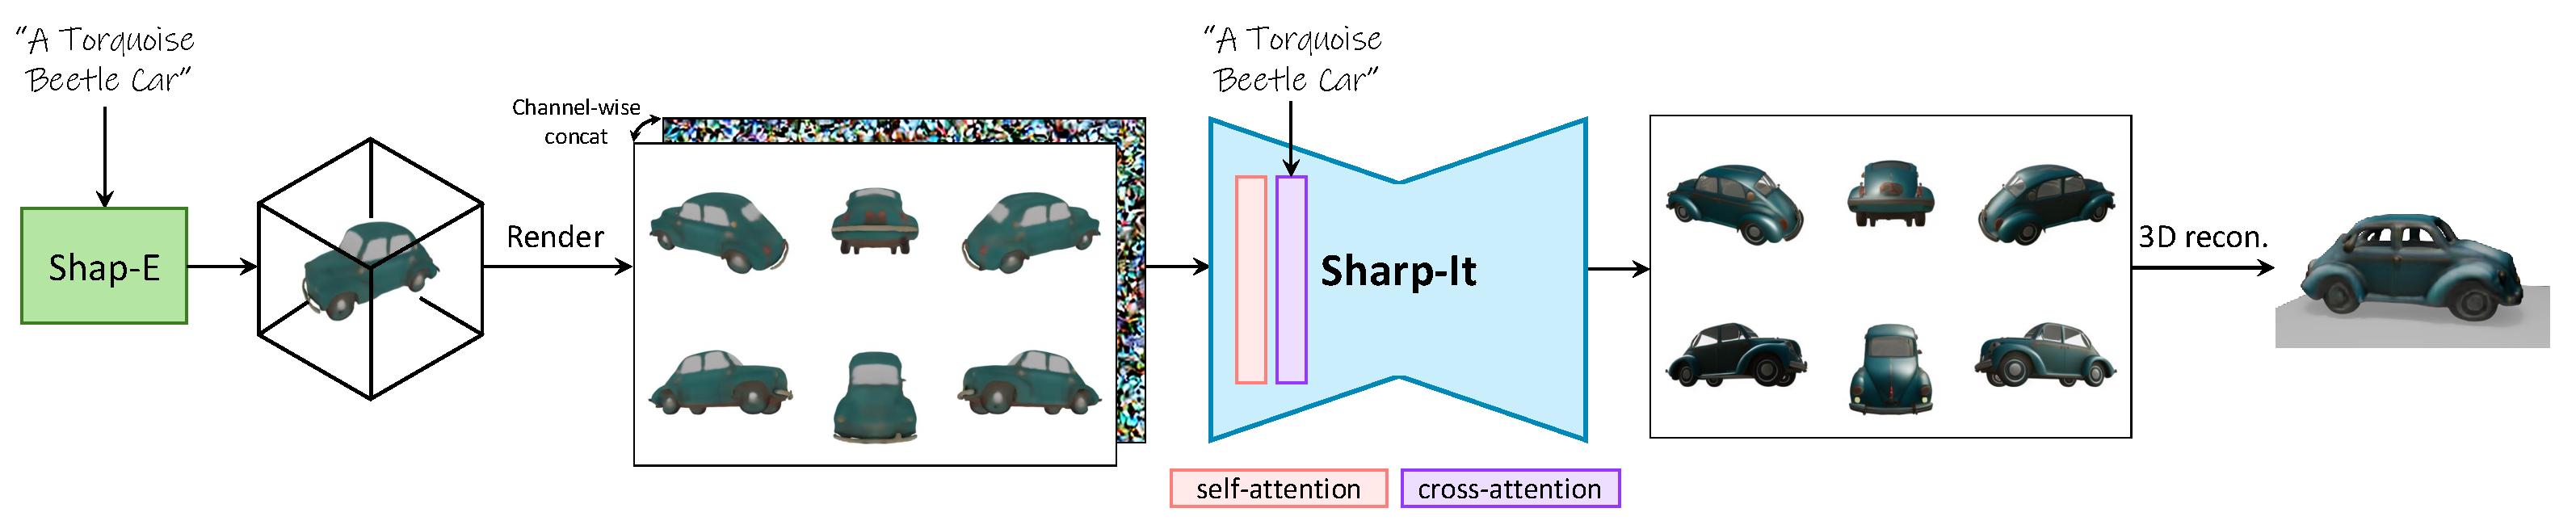
\includegraphics[width=\linewidth]{images/method_sharpe_new.pdf}
    \vspace{-18pt}
    \caption{Overview of 3D generation pipeline with Sharp-It.
    First, a 3D object is generated with Shap-E. Then, we render six views of this low-quality object. Sharp-It is a diffusion model based on Stable Diffusion~\cite{rombach2022highresolutionimagesynthesislatent} that enhances these views with the guidance of a text prompt by refining geometry and adding detailed appearance. Sharp-It employs cross-attention layers for text-based guidance and self-attention layers for cross-view consistency. A high-quality 3D object can be reconstructed from the multi-view image set.}
    \vspace{-12pt}
    \label{fig:method}
\end{figure*}
\section{Method}
In this section, we present our approach to addressing the quality gap between direct 3D generative models and those that reconstruct 3D objects from multi-view images.
We focus on Shap-E~\cite{jun2023shape}, a 3D generative model, and introduce \emph{\ourname}, a multi-view-to-multi-view diffusion model that enhances 3D objects generated by Shap-E. We train \ourname{} to improve these objects by adding intricate appearance details and correcting geometric artifacts such as discontinuities and broken parts.
% We begin by providing the necessary background on Shap-E and Zero123++, the diffusion models upon which \ourname{} builds.
The process of generating a 3D model with \ourname{} is demonstrated in Figure~\ref{fig:method}.

\subsection{Preliminaries}

\paragraph{Shap-E} 
is a latent diffusion model specifically designed for generating 3D assets. As common in latent diffusion models~\cite{rombach2022highresolutionimagesynthesislatent}, Shap-E is trained in two stages. In the first stage, an encoder is trained to map 3D objects into a latent space. This latent space corresponds to the weight space of implicit functions that represent 3D shapes, with each shape represented as an element in $\mathbb{R}^{1024\times1024}$. The latent representation can be decoded using Signed Texture Field (STF) rendering, where it is treated as the weights of an implicit function.
In the second stage, a diffusion model is trained within the Shap-E latent space, allowing for conditioning on either text or images.

\paragraph{Zero123++}
is an image-conditioned diffusion model designed to generate 3D-consistent multi-view images from a single input view~\cite{shi2023zero123singleimageconsistent}
. It builds upon Stable Diffusion~\cite{rombach2022highresolutionimagesynthesislatent}, which is a latent diffusion model comprising a VAE and a UNet. The VAE encodes images into a resolution that is eight times smaller and consists of four channels, while the UNet serves as the diffusion model, operating on the four-channel latent codes.
Zero123++ is a fine-tuned version of Stable Diffusion that accepts an image as input. Given an input image, it produces a $3\times2$ grid of $320\times320$ pixel images, with six constant azimuth and elevation angles. 
Originally, Zero123++~\cite{shi2023zero123singleimageconsistent} was designed to generate this grid image with a grey background. In InstantMesh~\cite{xu2024instantmesh}, it was further fine-tuned to render a white background, addressing the issue of ``floaties''—particles floating through space during 2D-to-3D lifting.

\subsection{Dataset Construction} \label{sec:data}
We begin by constructing a paired dataset consisting of degraded Shap-E objects along with corresponding high-quality objects. Our key idea in constructing the dataset is that such pairs can be obtained by employing the encoder of Shap-E in conjunction with a high-quality 3D objects dataset.
Specifically, we utilize objects from Objaverse~\cite{deitke2023objaversexluniverse10m3d}, provided by~\cite{luo2023scalable, luo2024view}, and encode them using Shap-E's encoder. For each pair of an object from Objaverse and its encoded Shap-E latent code, we render a $3\times2$ grid from six predefined camera views, applying three HDR lighting conditions. Our experiments, detailed in the ablation studies, indicate that rendering each object under varying HDR lighting enhances the model’s performance.

We apply a filtering criteria on the resulting dataset.
We remove objects where the degraded Shap-E rendering is significantly different from the original object's rendering, indicating a failure of Shap-E's encoder. Additionally, we filter out objects that are too thin or do not match certain keywords based on their annotated captions. For each remaining object, we extract a caption using BLIP2~\cite{li2023blip2}.
Finally, we split the dataset into training and test sets, resulting in 180,000 objects for training and 6,000 for testing.


\subsection{\ourname}
\ourname{} is a multi-view to multi-view diffusion model designed to enhance low-quality multi-view images of 3D objects generated by Shap-E. It takes as input a set of multi-view images rendered from a low-quality 3D object, along with a textual prompt, and produces high-quality multi-view images with refined geometric details and textures that correspond to the input views.
% In practice, the multi-view image set is organized as a grid of $3\times2$ views, resulting in a total resolution of $960\times640$. Each view has its own azimuth and elevation angles, which remain fixed across different objects. 
An overview of a 3D generation pipeline with \ourname{} is shown in Figure~\ref{fig:method}.

\paragraph{Architecture}
The architecture of \ourname{} has two key requirements: generating multi-view image sets and incorporating input multi-view sets as conditions. We build on Zero123++~\cite{shi2023zero123singleimageconsistent, xu2024instantmesh}, which was fine-tuned for multi-view generation, where images are arranged in a $3\times2$ grid with a total resolution of $960\times640$ and fixed camera angles across objects.
%
To enable multi-view conditioning, we modify the architecture of Zero123++ by expanding the UNet input to 8 channels: 4 for latent noise and 4 for the VAE-encoded Shap-E multi-view images. This design lets our model leverage the coarse geometry from the input views to achieve better 3D consistency, and is inspired by image editing techniques that fine-tune diffusion models to accept an image as input and modify specific parts while preserving others~\cite{brooks2022instructpix2pix, rombach2022highresolutionimagesynthesislatent, yang2022paint}. Unlike these approaches, which operate on a single image, our model learns to enhance the input views in a 3D consistent manner. 
Furthermore, we replace Zero123++'s image embedding with text prompts in the cross-attention layers, enabling better enhancement control and appearance editing capabilities (Section~\ref{sec:app-edit}).


The model we build on consists of self-attention layers, which play an important role in facilitating the consistency of our produced multi-view set~\cite{shi2024mvdream, wang2023imagedream}. Since our model operates on a multi-view image grid, these layers can be seen as an application of cross-view attention between the different views. Similarly to previous works~\cite{wang2023imagedream, shi2024mvdream, shi2023zero123singleimageconsistent}, this allows our model to simultaneously refine corresponding points across different views by learning the correspondences between them. 
We visualize the learned correspondences in Figure~\ref{fig:cross-view-attention}. The figure displays self-attention maps for a query point marked by a red dot in the leftmost image. The results demonstrate that this point on the wheel receives the highest attention weight across different views. Additionally, the attention mechanism identifies semantically similar points -- notably, other wheels of the car.

\begin{figure*}[t]
  %--- zero-width box that is shifted slightly left ---%
  \makebox[0pt][l]{\hspace*{\shift}%

    %------------- actual content -------------%
    \setlength{\tabcolsep}{3pt}
    \scriptsize
    \begin{tabular}{ccccccccc}
        & Input (Shap-E) & GaussianDreamer & MVEdit & MVDream w/ &
          Zero123++ w/ & Zero123++ w/ & Zero123++ w/ & Ours (Sharp-It)\\
        &                &                &         & SDEdit &
          SDEdit (U) & SDEdit (C) & SDEdit (R) \\[2pt]

        % avocado couch ---------------------------------------------------- %
        \raisebox{43pt}{\multirow{2}{*}{%
          \rotlabel{``An avocado shaped\\leather couch''}}} &
        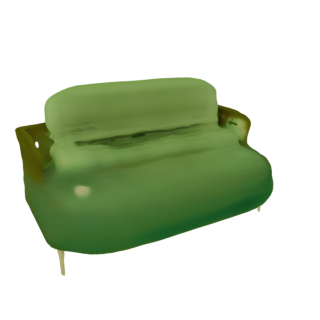
\includegraphics[width=\imgW]{images/comparison_plot/avocado_couch/shap-e/avocado_couch_view1_shap_e.png} &
        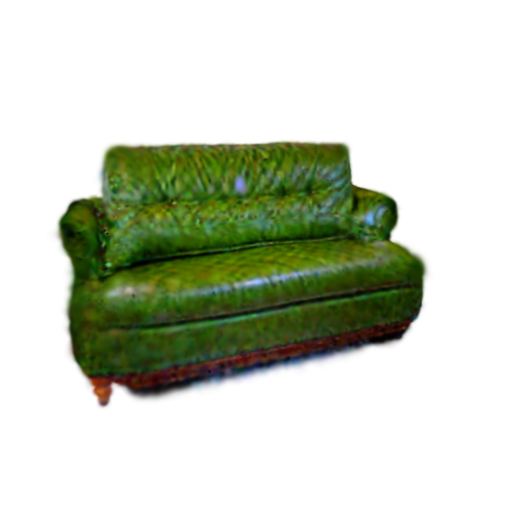
\includegraphics[width=\imgW,trim=30 30 30 30,clip]{images/comparison_plot/avocado_couch/gaussian_dreamer/1.png} &
        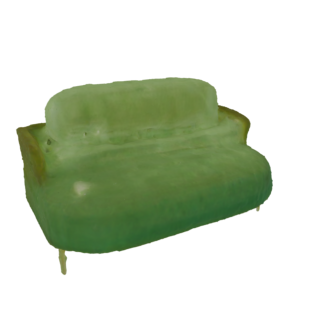
\includegraphics[width=\imgW]{images/comparison_plot/avocado_couch/mvedit/1.png} &
        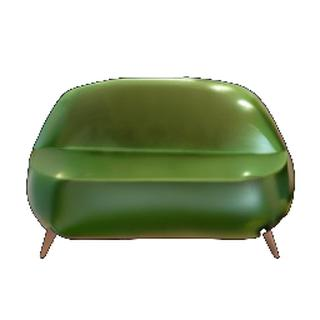
\includegraphics[width=\imgW]{images/comparison_plot/avocado_couch/mvdream/avo_couch_upscaled_3.jpg} &
        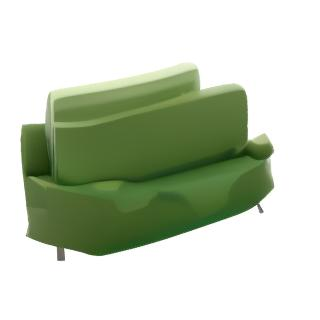
\includegraphics[width=\imgW]{images/comparison_plot/avocado_couch/zero123++/avo_couch_tile_2_3.jpg} &
        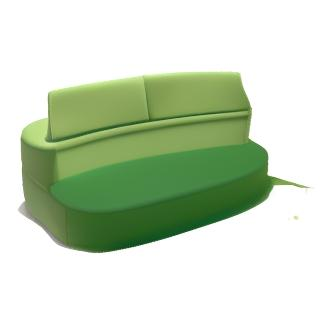
\includegraphics[width=\imgW]{images/comparison_plot/avocado_couch/zero123++image/avo_couch_tile_1_3.jpg} &
        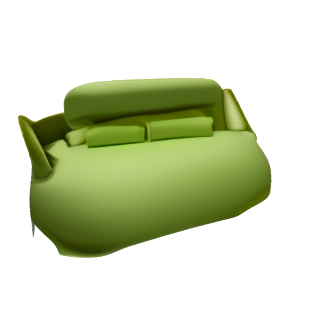
\includegraphics[width=\imgW]{images/comparison_plot/avocado_couch/zero123++refiner/split_image_0_2.png} &
        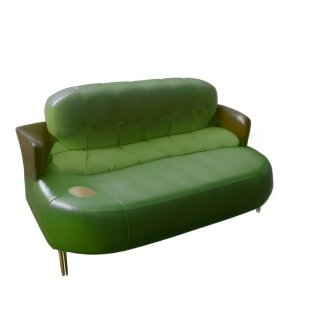
\includegraphics[width=\imgW]{images/comparison_plot/avocado_couch/sharp-e/avocado_couch_view1_sharp_e.png} \\

        & % second couch row
        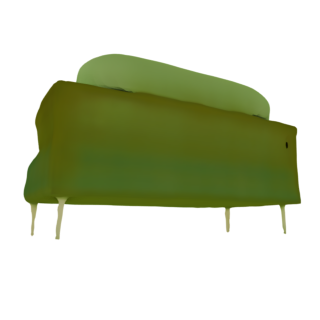
\includegraphics[width=\imgW]{images/comparison_plot/avocado_couch/shap-e/avocado_couch_view2_shap_e.png} &
        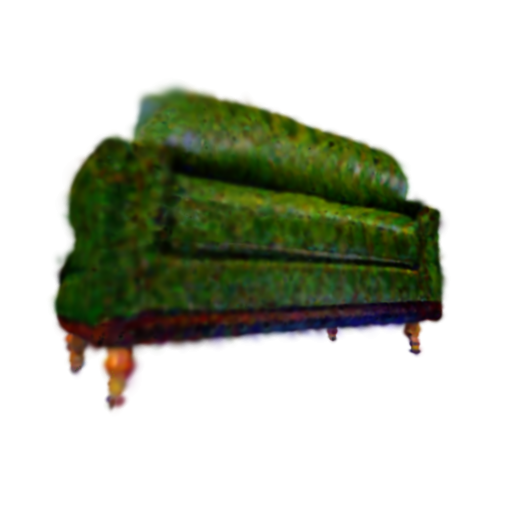
\includegraphics[width=\imgW,trim=30 30 30 30,clip]{images/comparison_plot/avocado_couch/gaussian_dreamer/3.png} &
        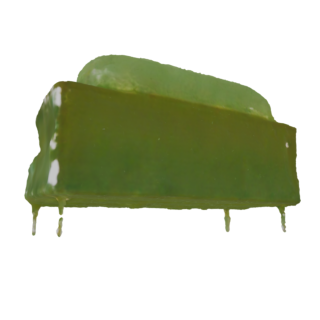
\includegraphics[width=\imgW]{images/comparison_plot/avocado_couch/mvedit/2.png} &
        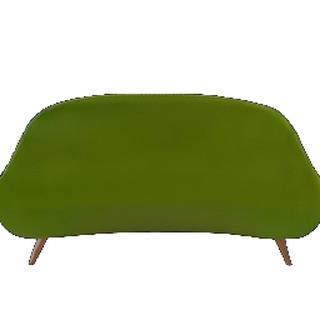
\includegraphics[width=\imgW]{images/comparison_plot/avocado_couch/mvdream/avo_couch_upscaled_1.jpg} &
        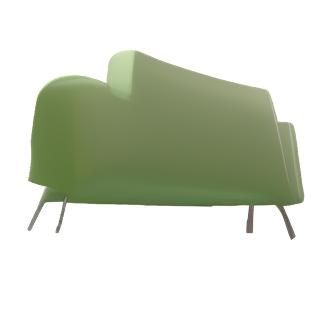
\includegraphics[width=\imgW]{images/comparison_plot/avocado_couch/zero123++/avo_couch_tile_2_6.jpg} &
        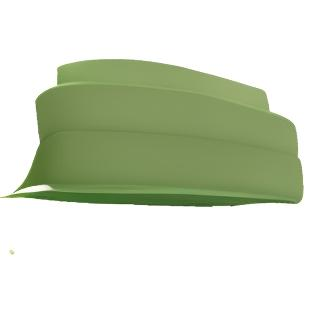
\includegraphics[width=\imgW]{images/comparison_plot/avocado_couch/zero123++image/avo_couch_tile_1_6.jpg} &
        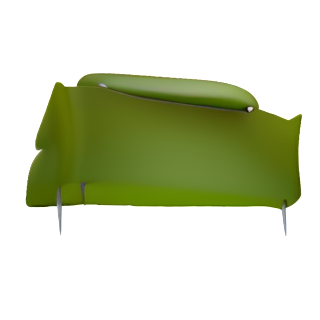
\includegraphics[width=\imgW]{images/comparison_plot/avocado_couch/zero123++refiner/split_image_0_5.png} &
        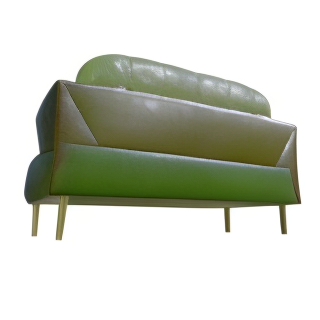
\includegraphics[width=\imgW]{images/comparison_plot/avocado_couch/sharp-e/avocado_couch_view2_sharp_e.png} \\[2pt]

        % bust -------------------------------------------------------------- %
        \raisebox{36pt}{\multirow{2}{*}{%
          \rotlabel{``A bust of a man\\with a beard''}}} &
        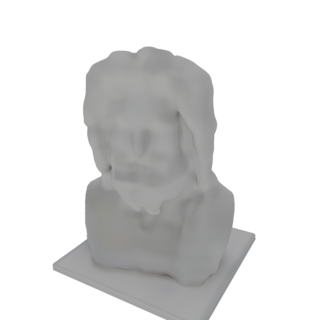
\includegraphics[width=\imgW]{images/comparison_plot/bust/shap-e/tile_0.png} &
        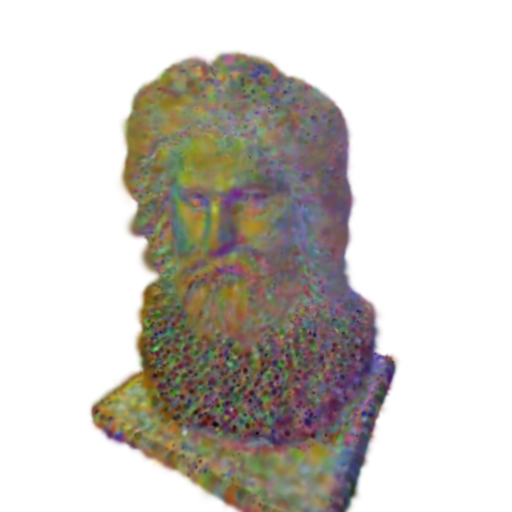
\includegraphics[width=\imgW]{images/comparison_plot/bust/gaussian_dreamer/0.png} &
        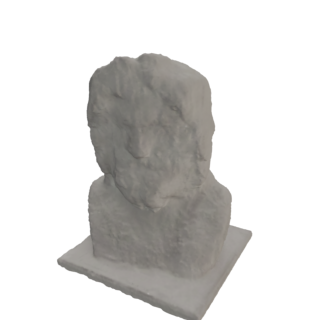
\includegraphics[width=\imgW]{images/comparison_plot/bust/mvedit/1.png} &
        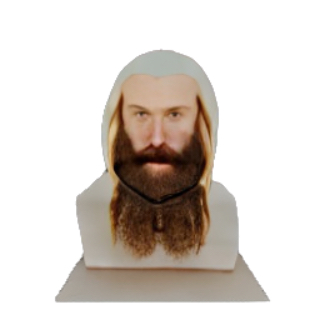
\includegraphics[width=\imgW]{images/comparison_plot/bust/mvdream/white_tile1.jpg} &
        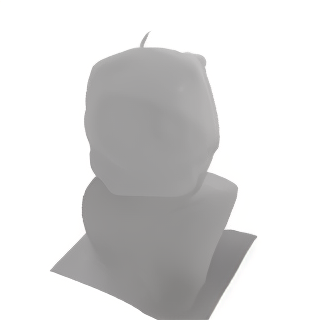
\includegraphics[width=\imgW]{images/comparison_plot/bust/zero123++/efbb32609fd44a4f849015e875bc57a1_tile_1.png} &
        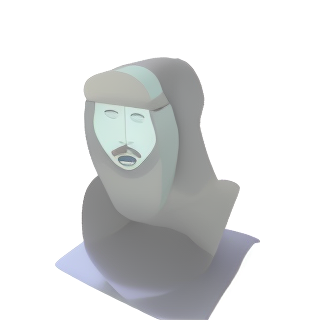
\includegraphics[width=\imgW]{images/comparison_plot/bust/zero123++img/efbb32609fd44a4f849015e875bc57a1_tile_1.png} &
        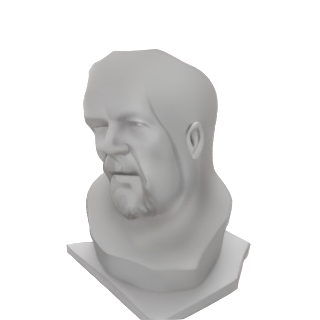
\includegraphics[width=\imgW]{images/comparison_plot/bust/zero123++refiner/split_image_1_0.png} &
        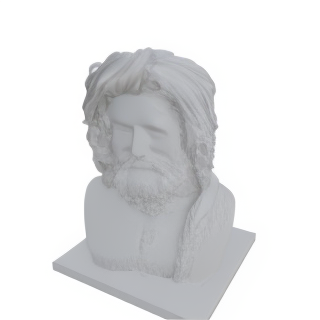
\includegraphics[width=\imgW]{images/comparison_plot/bust/sharp-e/efbb32609fd44a4f849015e875bc57a1_tile_1.png} \\

        & % second bust row
        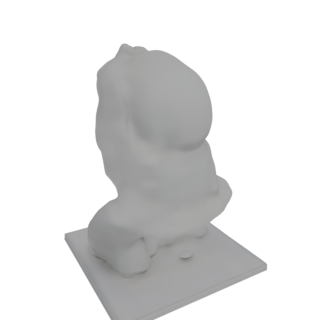
\includegraphics[width=\imgW]{images/comparison_plot/bust/shap-e/tile_2.png} &
        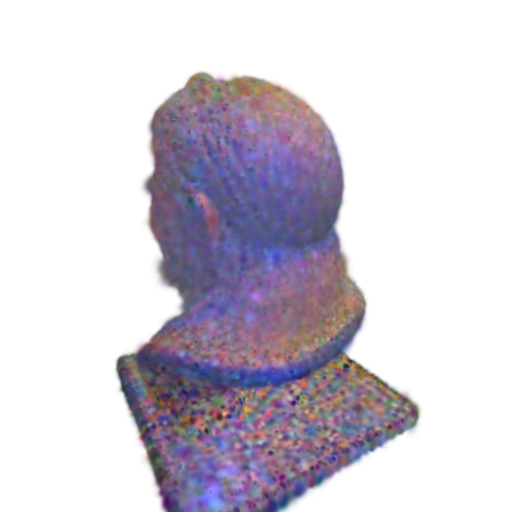
\includegraphics[width=\imgW]{images/comparison_plot/bust/gaussian_dreamer/bust_gaussian_dreamer_2.png} &
        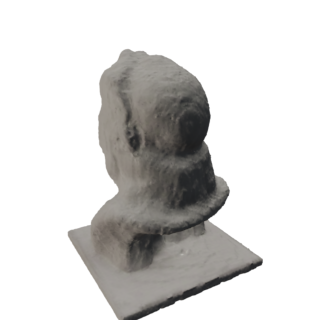
\includegraphics[width=\imgW]{images/comparison_plot/bust/mvedit/2.png} &
        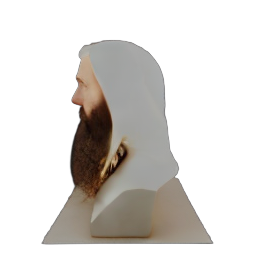
\includegraphics[width=\imgW]{images/comparison_plot/bust/mvdream/white_tile2.png} &
        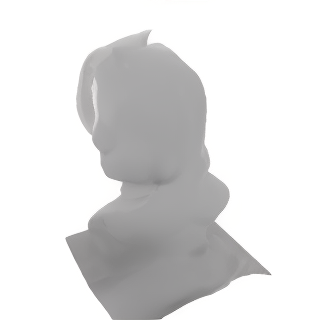
\includegraphics[width=\imgW]{images/comparison_plot/bust/zero123++/efbb32609fd44a4f849015e875bc57a1_tile_3.png} &
        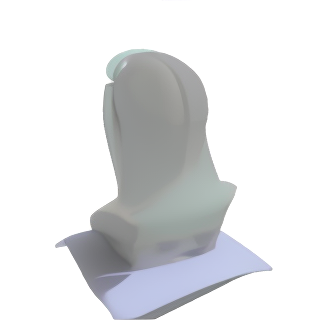
\includegraphics[width=\imgW]{images/comparison_plot/bust/zero123++img/efbb32609fd44a4f849015e875bc57a1_tile_3.png} &
        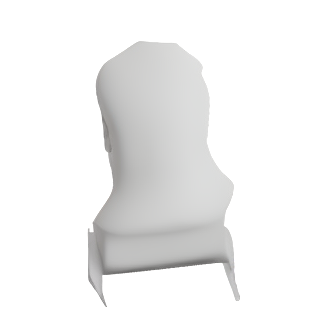
\includegraphics[width=\imgW]{images/comparison_plot/bust/zero123++refiner/split_image_1_2.png} &
        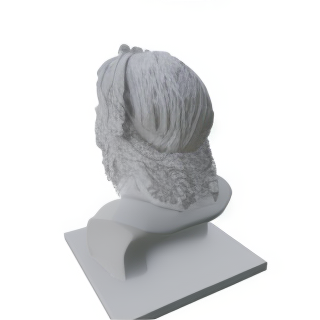
\includegraphics[width=\imgW]{images/comparison_plot/bust/sharp-e/efbb32609fd44a4f849015e875bc57a1_tile_3.png} \\[2pt]

        % tiki mask --------------------------------------------------------- %
        \raisebox{25pt}{\multirow{2}{*}{%
          \rotlabel{``A wooden\\tiki mask''}}} &
        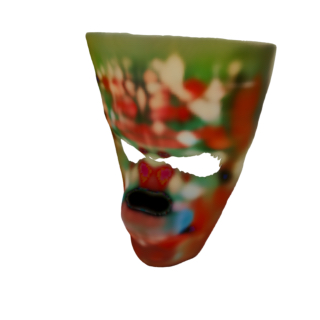
\includegraphics[width=\imgW]{images/comparison_plot/tiki_mask/shap-e/render_0000-4.jpg} &
        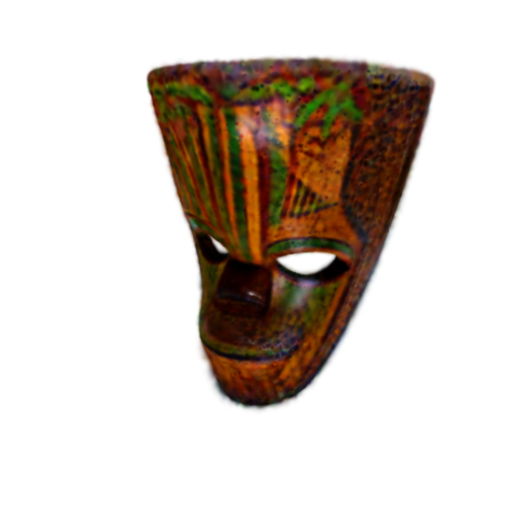
\includegraphics[width=\imgW]{images/comparison_plot/tiki_mask/gaussiandreamer/0.png} &
        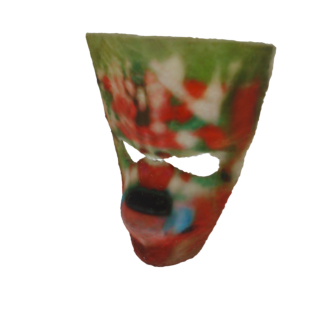
\includegraphics[width=\imgW]{images/comparison_plot/tiki_mask/mvedit/render_0000-3.jpg} &
        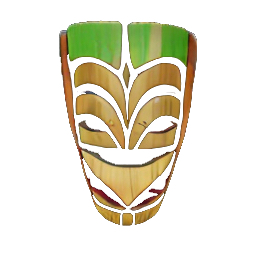
\includegraphics[width=\imgW]{images/comparison_plot/tiki_mask/mvdream/tile_0.jpg} &
        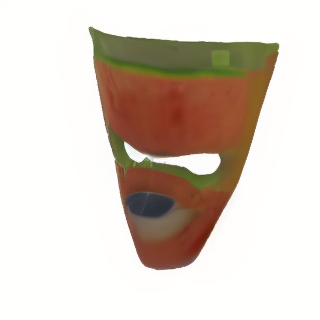
\includegraphics[width=\imgW]{images/comparison_plot/tiki_mask/zero123++unguided/avocado_couch_sdedit_steps_batch_0_tile_0.png} &
        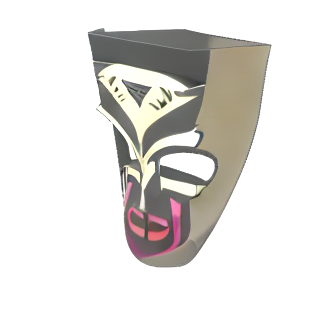
\includegraphics[width=\imgW]{images/comparison_plot/tiki_mask/zero123++guided/tiki_mask_guided_tile_0.png} &
        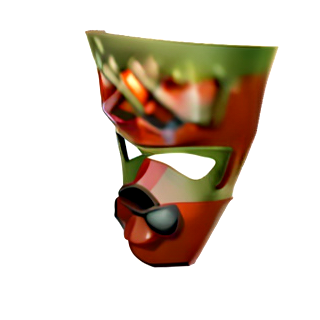
\includegraphics[width=\imgW]{images/comparison_plot/tiki_mask/zero123++refiner/split_image_2_0.png} &
        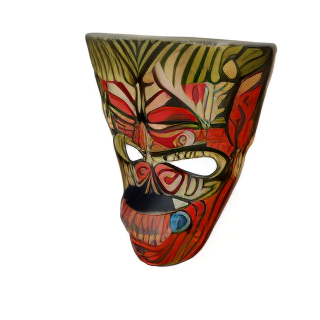
\includegraphics[width=\imgW]{images/comparison_plot/tiki_mask/sharp-e/10_75_steps_batch_0_a_wooden_tiki_mask_tile_0.png} \\

        & % second tiki row
        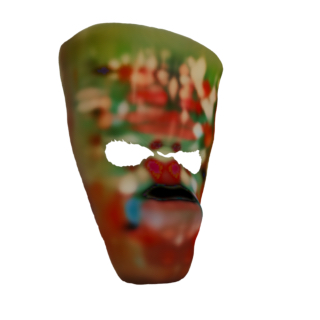
\includegraphics[width=\imgW]{images/comparison_plot/tiki_mask/shap-e/render_0005-2.jpg} &
        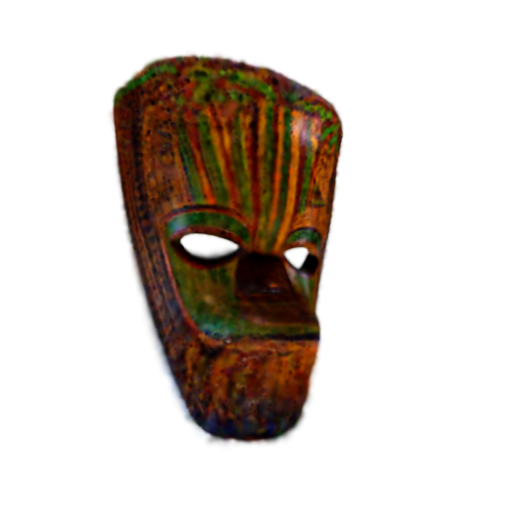
\includegraphics[width=\imgW]{images/comparison_plot/tiki_mask/gaussiandreamer/3.png} &
        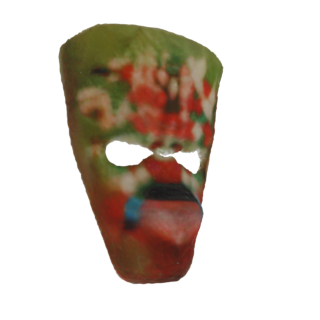
\includegraphics[width=\imgW]{images/comparison_plot/tiki_mask/mvedit/render_0005.jpg} &
        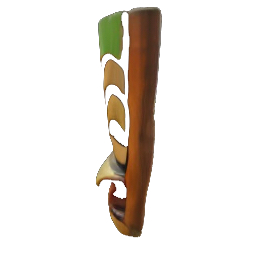
\includegraphics[width=\imgW]{images/comparison_plot/tiki_mask/mvdream/tile_1-2.jpg} &
        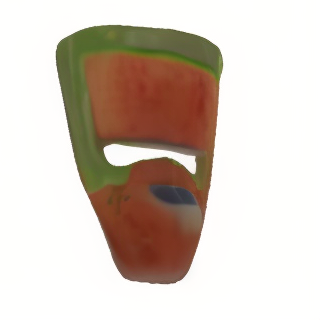
\includegraphics[width=\imgW]{images/comparison_plot/tiki_mask/zero123++unguided/avocado_couch_sdedit_steps_batch_0_tile_5.png} &
        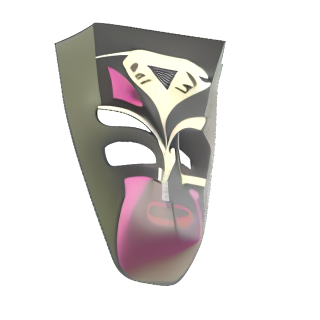
\includegraphics[width=\imgW]{images/comparison_plot/tiki_mask/zero123++guided/tiki_mask_guided_tile_5.png} &
        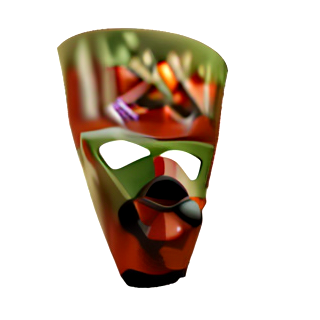
\includegraphics[width=\imgW]{images/comparison_plot/tiki_mask/zero123++refiner/split_image_2_5.png} &
        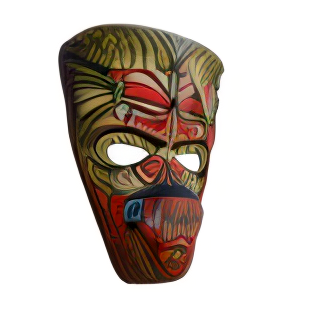
\includegraphics[width=\imgW]{images/comparison_plot/tiki_mask/sharp-e/10_75_steps_batch_0_a_wooden_tiki_mask_tile_5.png} \\
    \end{tabular}%
  }% end makebox

  \vspace{-12pt}
  \caption{%
    Comparison of Sharp-It with other methods for 3-D object enhancement.
    The first column shows the input generated by Shap-E; our method achieves
    the highest quality while best preserving the input.}
  \label{fig:mv2mv-comparisons}
\end{figure*}
\begin{table}[t]
    \caption{Quantitative comparison of our enhancement method with other baseline methods.}
    \vspace{-10pt}
    \label{tab:performance_comparison}
    \centering
    \setlength{\tabcolsep}{3pt} % Adjusts column padding for narrower width
    {\small % Keeps the font size at small
    \begin{tabular}{@{}lcccc@{}}
        \toprule
        \textbf{Method} & \textbf{FID $\downarrow$} & \textbf{CLIP $\uparrow$} & \textbf{DINO $\uparrow$} & \textbf{Runtime} \\ 
        \midrule
        GaussianDreamer & 50.89 & 0.81 & 0.82 &  6 min \\
        MVEdit & 44.87 & 0.83 & 0.77 &  1 min \\
        MVDream w/ SDEdit & 28.71 & 0.81 & 0.83 &  10 sec \\
        Zero123++ w/ SDEdit (U) & 24.59 & 0.87 & 0.86 &  10 sec \\
        Zero123++ w/ SDEdit (C) & 19.95 & 0.85 & 0.87 &  10 sec \\
        Zero123++ w/ SDEdit (R) & 19.13 & 0.87 & 0.89 &  10 sec \\
        Sharp-It & \textbf{6.60} & \textbf{0.90} & \textbf{0.92} &  10 sec \\
        \bottomrule
    \end{tabular}
    }
    \vspace{-12pt}
\end{table}

\begin{figure*}[t]
  %--- zero-width box that is shifted slightly left ---%
  \makebox[0pt][l]{\hspace*{\shift}%

    %------------- actual content -------------%
    \setlength{\tabcolsep}{3pt}
    \scriptsize
    \begin{tabular}{ccccccccc}
        & Input (Shap-E) & GaussianDreamer & MVEdit & MVDream w/ &
          Zero123++ w/ & Zero123++ w/ & Zero123++ w/ & Ours (Sharp-It)\\
        &                &                &         & SDEdit &
          SDEdit (U) & SDEdit (C) & SDEdit (R) \\[2pt]

        % avocado couch ---------------------------------------------------- %
        \raisebox{43pt}{\multirow{2}{*}{%
          \rotlabel{``An avocado shaped\\leather couch''}}} &
        \includegraphics[width=\imgW]{images/comparison_plot/avocado_couch/shap-e/avocado_couch_view1_shap_e.png} &
        \includegraphics[width=\imgW,trim=30 30 30 30,clip]{images/comparison_plot/avocado_couch/gaussian_dreamer/1.png} &
        \includegraphics[width=\imgW]{images/comparison_plot/avocado_couch/mvedit/1.png} &
        \includegraphics[width=\imgW]{images/comparison_plot/avocado_couch/mvdream/avo_couch_upscaled_3.jpg} &
        \includegraphics[width=\imgW]{images/comparison_plot/avocado_couch/zero123++/avo_couch_tile_2_3.jpg} &
        \includegraphics[width=\imgW]{images/comparison_plot/avocado_couch/zero123++image/avo_couch_tile_1_3.jpg} &
        \includegraphics[width=\imgW]{images/comparison_plot/avocado_couch/zero123++refiner/split_image_0_2.png} &
        \includegraphics[width=\imgW]{images/comparison_plot/avocado_couch/sharp-e/avocado_couch_view1_sharp_e.png} \\

        & % second couch row
        \includegraphics[width=\imgW]{images/comparison_plot/avocado_couch/shap-e/avocado_couch_view2_shap_e.png} &
        \includegraphics[width=\imgW,trim=30 30 30 30,clip]{images/comparison_plot/avocado_couch/gaussian_dreamer/3.png} &
        \includegraphics[width=\imgW]{images/comparison_plot/avocado_couch/mvedit/2.png} &
        \includegraphics[width=\imgW]{images/comparison_plot/avocado_couch/mvdream/avo_couch_upscaled_1.jpg} &
        \includegraphics[width=\imgW]{images/comparison_plot/avocado_couch/zero123++/avo_couch_tile_2_6.jpg} &
        \includegraphics[width=\imgW]{images/comparison_plot/avocado_couch/zero123++image/avo_couch_tile_1_6.jpg} &
        \includegraphics[width=\imgW]{images/comparison_plot/avocado_couch/zero123++refiner/split_image_0_5.png} &
        \includegraphics[width=\imgW]{images/comparison_plot/avocado_couch/sharp-e/avocado_couch_view2_sharp_e.png} \\[2pt]

        % bust -------------------------------------------------------------- %
        \raisebox{36pt}{\multirow{2}{*}{%
          \rotlabel{``A bust of a man\\with a beard''}}} &
        \includegraphics[width=\imgW]{images/comparison_plot/bust/shap-e/tile_0.png} &
        \includegraphics[width=\imgW]{images/comparison_plot/bust/gaussian_dreamer/0.png} &
        \includegraphics[width=\imgW]{images/comparison_plot/bust/mvedit/1.png} &
        \includegraphics[width=\imgW]{images/comparison_plot/bust/mvdream/white_tile1.jpg} &
        \includegraphics[width=\imgW]{images/comparison_plot/bust/zero123++/efbb32609fd44a4f849015e875bc57a1_tile_1.png} &
        \includegraphics[width=\imgW]{images/comparison_plot/bust/zero123++img/efbb32609fd44a4f849015e875bc57a1_tile_1.png} &
        \includegraphics[width=\imgW]{images/comparison_plot/bust/zero123++refiner/split_image_1_0.png} &
        \includegraphics[width=\imgW]{images/comparison_plot/bust/sharp-e/efbb32609fd44a4f849015e875bc57a1_tile_1.png} \\

        & % second bust row
        \includegraphics[width=\imgW]{images/comparison_plot/bust/shap-e/tile_2.png} &
        \includegraphics[width=\imgW]{images/comparison_plot/bust/gaussian_dreamer/bust_gaussian_dreamer_2.png} &
        \includegraphics[width=\imgW]{images/comparison_plot/bust/mvedit/2.png} &
        \includegraphics[width=\imgW]{images/comparison_plot/bust/mvdream/white_tile2.png} &
        \includegraphics[width=\imgW]{images/comparison_plot/bust/zero123++/efbb32609fd44a4f849015e875bc57a1_tile_3.png} &
        \includegraphics[width=\imgW]{images/comparison_plot/bust/zero123++img/efbb32609fd44a4f849015e875bc57a1_tile_3.png} &
        \includegraphics[width=\imgW]{images/comparison_plot/bust/zero123++refiner/split_image_1_2.png} &
        \includegraphics[width=\imgW]{images/comparison_plot/bust/sharp-e/efbb32609fd44a4f849015e875bc57a1_tile_3.png} \\[2pt]

        % tiki mask --------------------------------------------------------- %
        \raisebox{25pt}{\multirow{2}{*}{%
          \rotlabel{``A wooden\\tiki mask''}}} &
        \includegraphics[width=\imgW]{images/comparison_plot/tiki_mask/shap-e/render_0000-4.jpg} &
        \includegraphics[width=\imgW]{images/comparison_plot/tiki_mask/gaussiandreamer/0.png} &
        \includegraphics[width=\imgW]{images/comparison_plot/tiki_mask/mvedit/render_0000-3.jpg} &
        \includegraphics[width=\imgW]{images/comparison_plot/tiki_mask/mvdream/tile_0.jpg} &
        \includegraphics[width=\imgW]{images/comparison_plot/tiki_mask/zero123++unguided/avocado_couch_sdedit_steps_batch_0_tile_0.png} &
        \includegraphics[width=\imgW]{images/comparison_plot/tiki_mask/zero123++guided/tiki_mask_guided_tile_0.png} &
        \includegraphics[width=\imgW]{images/comparison_plot/tiki_mask/zero123++refiner/split_image_2_0.png} &
        \includegraphics[width=\imgW]{images/comparison_plot/tiki_mask/sharp-e/10_75_steps_batch_0_a_wooden_tiki_mask_tile_0.png} \\

        & % second tiki row
        \includegraphics[width=\imgW]{images/comparison_plot/tiki_mask/shap-e/render_0005-2.jpg} &
        \includegraphics[width=\imgW]{images/comparison_plot/tiki_mask/gaussiandreamer/3.png} &
        \includegraphics[width=\imgW]{images/comparison_plot/tiki_mask/mvedit/render_0005.jpg} &
        \includegraphics[width=\imgW]{images/comparison_plot/tiki_mask/mvdream/tile_1-2.jpg} &
        \includegraphics[width=\imgW]{images/comparison_plot/tiki_mask/zero123++unguided/avocado_couch_sdedit_steps_batch_0_tile_5.png} &
        \includegraphics[width=\imgW]{images/comparison_plot/tiki_mask/zero123++guided/tiki_mask_guided_tile_5.png} &
        \includegraphics[width=\imgW]{images/comparison_plot/tiki_mask/zero123++refiner/split_image_2_5.png} &
        \includegraphics[width=\imgW]{images/comparison_plot/tiki_mask/sharp-e/10_75_steps_batch_0_a_wooden_tiki_mask_tile_5.png} \\
    \end{tabular}%
  }% end makebox

  \vspace{-12pt}
  \caption{%
    Comparison of Sharp-It with other methods for 3-D object enhancement.
    The first column shows the input generated by Shap-E; our method achieves
    the highest quality while best preserving the input.}
  \label{fig:mv2mv-comparisons}
\end{figure*}
\begin{table}[t]
    \caption{Quantitative comparison of our enhancement method with other baseline methods.}
    \vspace{-10pt}
    \label{tab:performance_comparison}
    \centering
    \setlength{\tabcolsep}{3pt} % Adjusts column padding for narrower width
    {\small % Keeps the font size at small
    \begin{tabular}{@{}lcccc@{}}
        \toprule
        \textbf{Method} & \textbf{FID $\downarrow$} & \textbf{CLIP $\uparrow$} & \textbf{DINO $\uparrow$} & \textbf{Runtime} \\ 
        \midrule
        GaussianDreamer & 50.89 & 0.81 & 0.82 &  6 min \\
        MVEdit & 44.87 & 0.83 & 0.77 &  1 min \\
        MVDream w/ SDEdit & 28.71 & 0.81 & 0.83 &  10 sec \\
        Zero123++ w/ SDEdit (U) & 24.59 & 0.87 & 0.86 &  10 sec \\
        Zero123++ w/ SDEdit (C) & 19.95 & 0.85 & 0.87 &  10 sec \\
        Zero123++ w/ SDEdit (R) & 19.13 & 0.87 & 0.89 &  10 sec \\
        Sharp-It & \textbf{6.60} & \textbf{0.90} & \textbf{0.92} &  10 sec \\
        \bottomrule
    \end{tabular}
    }
    \vspace{-12pt}
\end{table}

\section{Experiments}
In this section, we evaluate the performance of \ourname{} in enhancing 3D objects generated by Shap-E. We compare our method against several baselines, conduct ablation studies to analyze the impact of different components, and demonstrate applications in 3D generation and editing.

\subsection{Qualitative and Quantitative Comparison}


\paragraph{Baselines}

We compare \ourname{} with various enhancement baselines. First, we compare against an SDS-based approach that was used in Spice-E~\cite{sella2024spicee}. Specifically, we use GaussianDreamer~\cite{yi2024gaussiandreamerfastgenerationtext}, initializing Gaussian Splatting with Shap-E's shape output and optimizing it with a text-to-image model. 
To make refining the thousands of objects in our test set practical, we limit the optimization time to six minutes per object.
We also include MVEdit~\cite{mvedit2024}, a multi-view editing method that  refines coarse 3D shapes.

\vspace{-10pt}
Another set of baselines combines multi-view image generation with SDEdit~\cite{meng2022sdedit}. Here, we render Shap-E’s shape into a multi-view image set and apply simultaneous edits across views to ensure consistency. Using SDEdit with a strength of 0.4, we add noise to each multi-view image and denoise it. For multi-view generation, we use both MVDream~\cite{shi2024mvdream}, which is guided by a text prompt, and Zero123++~\cite{shi2023zero123singleimageconsistent}, which is conditioned on an image rather than text.
With Zero123++, we test three configurations:
(i) Zero123++ w/ SDEdit (R), where we apply SDXL Refiner model (default strength value)~\cite{podell2023sdxlimprovinglatentdiffusion} on the frontal view of the object, and use this edited view to guide SDEdit across the multi-view set, (ii) Zero123++ w/ SDEdit (C), where SDEdit with Stable Diffusion (strength 0.75) is applied on the object's frontal view which is used to guide the multi-view SDEdit; and (iii) Zero123++ w/ SDEdit (U), where no image condition is used.
 

\vspace{-10pt}
\paragraph{Dataset}
We conduct our quantitative experiments on our test set described in Section~\ref{sec:data}.
% a subset of Objaverse~\cite{deitke2023objaversexluniverse10m3d} that was held out during the training of \ourname. Each object in this subset is first encoded into Shap-E's latent space and then enhanced using each method. 
To demonstrate our method's generalization capability, we also present results on objects generated directly by Shap-E from text prompts.

\vspace{-12pt}
\paragraph{Metrics}
To assess enhancement performance, we evaluate the image quality produced by each method. Specifically, we compute the FID~\cite{parmar2021cleanfid, heusel2017gans} between the enhanced views and our test set. Additionally, we evaluate the semantic and visual similarity of the enhanced shape with the ground-truth using CLIP~\cite{radford2021learning} and DINO~\cite{caron2021emerging} image encoders.

\vspace{-12pt}
\paragraph{Results}
We present a qualitative comparison in Figure~\ref{fig:mv2mv-comparisons}. The avocado couch and the tiki mask were generated by Shap-E, while the bust is an encoded object from the test set. As shown, our method preserves the objects' coarse details while producing high-quality, detailed enhancements. In contrast, other methods diverge significantly from the original objects and yield less realistic results. For instance, our method accurately generates a leather-like texture, whereas other methods struggle to enhance the flat appearance of the Shap-E-generated couch.
Our approach also maintains color consistency with the input shapes. This is evident in the couch's back section, where brown and green tints are faithfully preserved, as well as in the bust and tiki mask. Our method generates significantly more fine details compared to other methods, particularly visible in the intricate features of the bust and the textural elements of the mask. 
Results for the objects lifted to 3D are provided in the supplementary materials.
% Additional lifted results for each method are provided in the supplementary materials.

Quantitative comparisons are shown in Table~\ref{tab:performance_comparison}. Our method achieves the lowest FID, confirming it produces the highest-quality results. Furthermore, our method shows the best alignment with the ground-truth object, as indicated by the CLIP and DINO similarity metrics, The runtime of our method is comparable to or faster than other methods.



\subsection{Ablation Studies}


\begin{figure}
    \centering
    \setlength{\tabcolsep}{1pt}
    {\small
    \begin{tabular}{ccccc}
        & Input & W/o text  & W/o diverse & Full method \\
        && prompt & lighting \\
        %
        \raisebox{35pt}{\rotatebox[origin=c]{90}{View 1}} &
        \multicolumn{1}{c}{\includegraphics[width=0.24\linewidth, trim=50 0 50 0, clip]{images/ablation_plot/shap_e/mv_0_image_tile_1.png}} &
        \includegraphics[width=0.24\linewidth, trim=50 0 50 0, clip]{images/ablation_plot/no_prompt/no_prompt_tile_1.png} &
        \includegraphics[width=0.24\linewidth, trim=50 0 50 0, clip]{images/ablation_plot/single_hdr/single_source_tile_1.png} &
        \includegraphics[width=0.24\linewidth, trim=50 0 50 0, clip]{images/ablation_plot/full/full_tile_1.png} \\
        %
        \raisebox{35pt}{\rotatebox[origin=c]{90}{View 2}} &
        \multicolumn{1}{c}{\includegraphics[width=0.24\linewidth, trim=50 0 50 0, clip]{images/ablation_plot/shap_e/mv_0_image_tile_2.png}} &
        \includegraphics[width=0.24\linewidth, trim=50 0 50 0, clip]{images/ablation_plot/no_prompt/no_prompt_tile_2.png} &
        \includegraphics[width=0.24\linewidth, trim=50 0 50 0, clip]{images/ablation_plot/single_hdr/single_source_tile_2.png} &
        \includegraphics[width=0.24\linewidth, trim=50 0 50 0, clip]{images/ablation_plot/full/full_tile_2.png} \\
        %
        \raisebox{35pt}{\rotatebox[origin=c]{90}{View 3}} &
        \multicolumn{1}{c}{\includegraphics[width=0.24\linewidth, trim=50 0 50 0, clip]{images/ablation_plot/shap_e/mv_0_image_tile_5.png}} &
        \includegraphics[width=0.24\linewidth, trim=50 0 50 0, clip]{images/ablation_plot/no_prompt/no_prompt_tile_5.png} &
        \includegraphics[width=0.24\linewidth, trim=50 0 50 0, clip]{images/ablation_plot/single_hdr/single_source_tile_5.png} &
        \includegraphics[width=0.24\linewidth, trim=50 0 50 0, clip]{images/ablation_plot/full/full_tile_5.png} \\
        %
        \multicolumn{5}{c}{``A knight in full plate armor''}
    \end{tabular}
    }
    \caption{Qualitative ablation study. The first column shows the degraded input object generated by Shap-E. Subsequent columns show the effects of removing specific components: omitting the text prompt leads to reduced texture detail, while excluding diverse lighting results in a flatter appearance with less realistic shading. The full model achieves the most refined and detailed result.}
    \label{fig:ablation}
\end{figure}


We conduct ablation studies to assess the contributions of different components in \ourname. 
First, we examine the importance of using an input text prompt, which is not utilized in Zero123++~\cite{shi2023zero123singleimageconsistent, xu2024instantmesh}, the model upon which we build.
Second, we explore the effect of constructing the dataset with diverse lighting conditions, rather than using a single type of lighting.
% Specifically, we examine the importance of using an input text prompt and the effect of constructing the dataset with diverse lighting conditions. 

For this analysis, we train our method without each component individually and present the results in Figure~\ref{fig:ablation}.
For computational efficiency, ablation models (including the full method one) were trained for 400,000 steps, fewer than in our main experiments.
\begin{table}[ht]
    \centering
    \caption{Quantitative results of our ablation study. All models were trained for 400,000 steps.}
    \label{tab:ablation}
    \begin{tabular}{@{}lcccc@{}} % Align columns to the left
        \toprule
        \textbf{Ablation} & \textbf{FID $\downarrow$} & \textbf{CLIP $\uparrow$} & \textbf{DINO $\uparrow$}  \\ 
        \midrule
            W/o text prompt & 9.91 & \textbf{0.91} &0.91&  \\
        W/o diverse lighting  & 9.16 & 0.89 & 0.91 &  \\
        Full method & \textbf{8.06} & 0.89 & 0.91 \\

        \bottomrule
    \end{tabular}
    \vspace{-16pt}
\end{table}

In the first column, we show a shape generated by Shap-E, which serves as input to the models in the subsequent rows. In the second column, we omit the text prompt, instead using an empty prompt. As shown, without a guiding text prompt, the results lack detail and fail to achieve a metallic appearance. In the third column, we construct the dataset with a single lighting condition, leading to a notable enhancement of the input shape but still lacking finer details. The last column displays results from our full model, which successfully achieves a metallic look and produces highly detailed shapes. Importantly, our results are consistent with the coarse details of the input shape. The lifted object of this example is included in the supplementary materials.
We also quantitatively evaluate each configuration using the metrics described in the previous section. Results are provided in Table~\ref{tab:ablation}. While all configurations are comparable aligned with the ground truth object, the full model achieves the highest image quality.


\begin{figure*}
\centering

\setlength{\tabcolsep}{1pt}
{\small
\begin{tabular}{c c c c c c c c c}
    & \multicolumn{2}{c}{``A Gundam''} & { } & \multicolumn{2}{c}{``A tank''} & { } & \multicolumn{2}{c}{``A glass and metal battle-axe''} \\
    %
    \raisebox{20pt}{\rotatebox[origin=c]{90}{Input}} &
    \includegraphics[width=0.13\linewidth]{images/generation_results/shap-e/gundam/gundam_tile_1.png} &
    \includegraphics[width=0.13\linewidth]{images/generation_results/zero123/gundam/gundam_solo.jpg} & { } & 
    \includegraphics[width=0.13\linewidth, trim=0 0 0 60, clip]{images/generation_results/shap-e/tank/tank_tile_2.png} &
    \includegraphics[width=0.13\linewidth, trim=0 50 0 150, clip]{images/generation_results/zero123/tank/tank_rem.jpg} & { } & 
    \includegraphics[width=0.13\linewidth]{images/generation_results/shap-e/glass_battle_axe/glass_battle_axe_tile_4.png} &
    \includegraphics[width=0.13\linewidth]{images/generation_results/zero123/glass_axe/glass_axe_14_rem.jpg}
    \\
    %
      \raisebox{20pt}{\rotatebox[origin=c]{90}{View 1}} &
    \includegraphics[width=0.13\linewidth]{images/generation_results/sharp-e/gundam/a_gundam_75_steps_batch_0_a_gundam_tile_2.png} &
    \includegraphics[width=0.13\linewidth]{images/generation_results/zero123/gundam/gundam_tile_0.jpg} & { } & 
    \includegraphics[width=0.13\linewidth, trim=20 50 20 50, clip]{images/generation_results/sharp-e/tank/a_battle_tank_75_steps_batch_0_a_battle_tank_tile_4.png} &
    \includegraphics[width=0.13\linewidth, trim=0 20 0 20, clip]{images/generation_results/zero123/tank/tank_tile_0.png} & { } & 
    \includegraphics[width=0.13\linewidth]{images/generation_results/sharp-e/axe/2_250_steps_batch_0_a_battle_axe_made_out_of_glass_tile_0.png} &
    \includegraphics[width=0.13\linewidth]{images/generation_results/zero123/glass_axe/glass_axe_14_tile_0.jpg}
    \\
    %
    \raisebox{20pt}{\rotatebox[origin=c]{90}{View 2}} &
    \includegraphics[width=0.13\linewidth]{images/generation_results/sharp-e/gundam/a_gundam_75_steps_batch_0_a_gundam_tile_1.png} &
    \includegraphics[width=0.13\linewidth]{images/generation_results/zero123/gundam/gundam_tile_1.jpg} & { } & 
    \includegraphics[width=0.13\linewidth, trim=0 0 0 60, clip]{images/generation_results/sharp-e/tank/a_battle_tank_75_steps_batch_0_a_battle_tank_tile_2.png} &
    \includegraphics[width=0.13\linewidth, trim=0 0 0 20, clip]{images/generation_results/zero123/tank/tank_tile_4.png} & { } & 
    \includegraphics[width=0.13\linewidth]{images/generation_results/sharp-e/axe/2_250_steps_batch_0_a_battle_axe_made_out_of_glass_tile_4.png} &
    \includegraphics[width=0.13\linewidth]{images/generation_results/zero123/glass_axe/glass_axe_14_tile_3.jpg} \\
    %
    & \multicolumn{1}{c}{Ours} & \multicolumn{1}{c}{Zero123++} & { } & \multicolumn{1}{c}{Ours} & \multicolumn{1}{c}{Zero123++} & { } & \multicolumn{1}{c}{Ours} & \multicolumn{1}{c}{Zero123++} \\
     
\end{tabular}
}
\vspace{-8pt}
\caption{
Text-to-MultiView qualitative results. Our method generates a multi-view set by creating a 3D object with Shap-E and refining it with \ourname. In contrast, Zero123++ first generates a single image with Stable Diffusion, then produces a multi-view set conditioned on that image. This approach leads to geometric artifacts, such as flatness (gundam) and the Janus problem (tank). Leveraging Shap-E's 3D knowledge, our method yields high-quality, coherent objects. Additional 3D renderings of these results are provided in the supplemental.
}
\vspace{-12pt}
\label{fig:text-to-3d}
\end{figure*}

\section{Applications}
We now demonstrate the various applications enabled by \ourname. Specifically, we show how \ourname{} bridges the quality gap between Shap-E and multi-view-based 3D generation methods, while supporting diverse 3D generative applications.


\vspace{-16pt}
\paragraph{Text-to-3D Generation}
As discussed in previous sections, a common approach for text-to-3D synthesis involves first generating a nearly consistent multi-view image set~\cite{shi2024mvdream, wang2023imagedream, shi2023zero123singleimageconsistent}, followed by a sparse-view 3D reconstruction method~\cite{xu2024instantmesh}. By combining Shap-E with \ourname, we achieve text-to-multi-view image synthesis, enabling a complete pipeline for 3D generation (Figure~\ref{fig:method}).
In Figure~\ref{fig:text-to-3d}, we compare text-to-multi-view results from Zero123++ and our method. Our method achieves results comparable to Zero123++ in terms of image quality, while demonstrating superior geometric details. The advantage of using Shap-E as a first stage is particularly evident in the tank and Gundam examples. The tank produced by Zero123++ suffers from a Janus problem, where wheels incorrectly appear on two adjacent sides. Moreover, Zero123++ generates a flat Gundam figure, lacking geometric details. These results demonstrate the effectiveness of our pipeline: using a 3D-aware model to generate a coarse 3D object, followed by refinement using an image diffusion model.


\vspace{-12pt}
\paragraph{3D Object Editing}

\begin{figure}
    \centering
    \setlength{\tabcolsep}{1pt}
    {\scriptsize
    \begin{tabular}{ccccc}
        %
        & \multicolumn{4}{c}{``A table lamp'' $\longrightarrow$ ``A golden table lamp''} \\
        %
        \raisebox{12pt}{\multirow{3}{*}{\rotatebox[origin=t]{90}{Shap-Editor}}} &
                \includegraphics[width=0.15\linewidth, trim=70 45 70 40, clip]
                % L B R T
{images/editings/shap-editor/lamps/original/render_0000.png} &
                       \includegraphics[width=0.15\linewidth, trim=70 45 70 40, clip]
{images/editings/shap-editor/lamps/shap_e/original_shap_e_tile_0.png} &
                        \includegraphics[width=0.15\linewidth, trim=70 45 70 40, clip]
{images/editings/shap-editor/lamps/edit1_shap_e/golden_shap_e_tile_0.png} &
                       \includegraphics[width=0.15\linewidth, trim=70 45 70 40, clip]
{images/editings/shap-editor/lamps/edit1_sharp_e/0_75_steps_batch_0_a_golden_table_lamp_tile_0.png} \\
        %
        %
        & \multicolumn{4}{c}{``A table lamp'' $\longrightarrow$ ``A santa table lamp''} \\
        %
         &
                       \includegraphics[width=0.15\linewidth, trim=70 45 70 40, clip]
{images/editings/shap-editor/lamps/original/render_0000.png} &
                      \includegraphics[width=0.15\linewidth, trim=70 45 70 40, clip]
{images/editings/shap-editor/lamps/shap_e/original_shap_e_tile_0.png} &
                    \includegraphics[width=0.15\linewidth, trim=70 45 70 40, clip]
{images/editings/shap-editor/lamps/edit2_shap_e/santa_0.png} &
                      \includegraphics[width=0.15\linewidth, trim=70 45 70 40, clip]
{images/editings/shap-editor/lamps/edit2_sharp_e/0_75_steps_batch_0_a_santa_table_lamp_tile_0.png} \\
        %
        %
        & \multicolumn{4}{c}{``A blue beetle car'' $\longrightarrow$ ``A torquoise beetle car''} \\
        %
                        % L B R T

        \raisebox{12pt}{\multirow{3}{*}{\rotatebox[origin=t]{90}{DDPM Inversion}}} &
    \includegraphics[width=0.22\linewidth, trim=30 60 15 85, clip]
{images/editings/ddpm_inv/original/render_0000.png} &
           \includegraphics[width=0.22\linewidth, trim=30 60 15 85, clip]{images/editings/ddpm_inv/shap_e/original_shap_e_tile_0.png} &
           \includegraphics[width=0.22\linewidth, trim=30 60 0 85, clip]{images/editings/ddpm_inv/edit1_shap_e/torquoise_shap_e_tile_0.png} &
           \includegraphics[width=0.22\linewidth, trim=30 60 0 85, clip]{images/editings/ddpm_inv/edit1_sharp_e/torquoise_beetle_car_75_steps_batch_0_a_matte_torquoise_beetle_car_tile_0.png} \\
        %
        %
         & \multicolumn{4}{c}{``A blue beetle car'' $\longrightarrow$ ``A blue SUV''} \\
        %
         &
             \includegraphics[width=0.22\linewidth, trim=30 60 15 85, clip]{images/editings/ddpm_inv/original/render_0000.png} &
            \includegraphics[width=0.22\linewidth, trim=30 60 15 85, clip]{images/editings/ddpm_inv/shap_e/original_shap_e_tile_0.png} &
           \includegraphics[width=0.22\linewidth, trim=30 60 0 85, clip]{images/editings/ddpm_inv/edit2_shap_e/mv_0_image_tile_0.png} &
               \includegraphics[width=0.22\linewidth, trim=30 60 0 85, clip]{images/editings/ddpm_inv/edit2_sharp_e/blue_suv_75_steps_batch_0_a_metalic_blue_suv_tile_0.png} \\
        %
        %
        & Input Shape & Encoded Shaped & Edit & + \ourname{}
    \end{tabular}
    }
    \vspace{-4pt}
    \caption{
    Our method enhances edits performed in Shap-E's space (rightmost column). We show editing results obtained with an existing editing method (Shap-Editor), and demonstrate that DDPM Inversion, originally developed for image diffusion models, works with Shap-E and can be integrated with \ourname{}.
    }
    \vspace{-16pt}
    \label{fig:edits}
\end{figure}
Shap-E provides a latent space in which semantic manipulation of 3D shapes can be performed while maintaining 3D consistency. Our method enhances these edited shapes to achieve high-quality objects. We demonstrate our method's application with two different editing techniques.
First, we use Shap-Editor~\cite{chen2023shapeditor}, which trains a model that takes a Shap-E latent code and a text instruction to produce a new latent code corresponding to the edited shape. While this method enables diverse and fast editing of 3D shapes, it is bounded by Shap-E's quality limitations. \ourname{} addresses this limitation by enhancing the results produced by Shap-Editor.
Second, inspired by diffusion-based editing methods for images, we apply a technique that enables shape editing with Shap-E. Specifically, we apply Edit-Friendly DDPM Inversion~\cite{huberman2024edit} with Shap-E instead of an image diffusion model.

Results for both methods are shown in Figure~\ref{fig:edits}. By combining \ourname{} with existing editing methods, we enable various types of high-quality 3D edits. These include changing an object's shape (demonstrated by transforming a car into an SUV), adding decorations (shown with the Christmas lamp), and modifying colors (as seen with the golden lamp and turquoise car).


\vspace{-16pt}
\paragraph{Appearance Editing} \label{sec:app-edit}
\ourname{} enables detailed control over the appearance of a degraded shape using text prompts. Specifically, at inference time, we can apply a different prompt from the one used during the generation of the Shap-E object, facilitating appearance editing that accurately preserves the original shape. Examples of this application are presented in Figures~\ref{fig:teaser} and \ref{fig:edits-appearance}.

% \begin{figure}
    \centering
    \setlength{\tabcolsep}{1pt}
    {\small
    \begin{tabular}{cccc}
        %
        \multicolumn{4}{c}{``Golden Jewelry Box'' $\longrightarrow$ ``Suede Leather Jewelry Box''} \\
        %
        \includegraphics[width=0.22\linewidth]{images/editings/appearance_edit/box/jewls_tile_0.png} &
        \includegraphics[width=0.22\linewidth]{images/editings/appearance_edit/box/jewls_tile_1.png} &
        \includegraphics[width=0.22\linewidth]{images/editings/appearance_edit/box/jewlery_jewlery_box_2_75_steps_batch_0_a_suede_leather_jewlry_box_tile_0.png} &
        \includegraphics[width=0.22\linewidth]{images/editings/appearance_edit/box/jewlery_jewlery_box_2_75_steps_batch_0_a_suede_leather_jewlry_box_tile_1.png} \\
        %
        \multicolumn{4}{c}{``Glass City Tower'' $\longrightarrow$ ``Wooden City Tower''} \\
        %
        \includegraphics[width=0.22\linewidth]{images/editings/appearance_edit/tower/glass_city_tower_tile_0.png} &
        \includegraphics[width=0.22\linewidth]{images/editings/appearance_edit/tower/glass_city_tower_tile_1.png} &
        \includegraphics[width=0.22\linewidth]{images/editings/appearance_edit/tower/glass_city_tower_2_75_steps_batch_0_a_wooden_city_tower_tile_0.png} &
        \includegraphics[width=0.22\linewidth]{images/editings/appearance_edit/tower/glass_city_tower_2_75_steps_batch_0_a_wooden_city_tower_tile_1.png} \\
        %
        \multicolumn{4}{c}{``Leather Chair'' $\longrightarrow$ ``Leopard Print Leather Chair''} \\
        %
        \includegraphics[width=0.22\linewidth]{images/editings/appearance_edit/chair/mv_0_image_tile_0.png} &
        \includegraphics[width=0.22\linewidth]{images/editings/appearance_edit/chair/mv_0_image_tile_1.png} &
        \includegraphics[width=0.22\linewidth]{images/editings/appearance_edit/chair/chair_test_2_75_steps_batch_0_a_leopard_print_leather_chair_tile_0.png} &
        \includegraphics[width=0.22\linewidth]{images/editings/appearance_edit/chair/chair_test_2_75_steps_batch_0_a_leopard_print_leather_chair_tile_1.png} \\
        %
        \multicolumn{2}{c}{Input} & \multicolumn{2}{c}{Appearance Edit}
    \end{tabular}
    }
    \vspace{-6pt}
    \caption{
    \ourname{} allows to edit the appearance of a Shap-E object by changing the prompt during the enhancement step. 
    }
    \vspace{-14pt}
    \label{fig:edits-appearance}
\end{figure}
\begin{figure}
    \centering
    \setlength{\tabcolsep}{1pt}
    {\small
    \begin{tabular}{cccc}
        %
        \multicolumn{4}{c}{``A red velvet chesterfield chair''} \\
        %
                \includegraphics[width=0.24\linewidth, trim=20 20 40 40, clip]{images/editings/spice-e/velvet_chair/guidance/chair_0000.jpg} &
                \includegraphics[width=0.24\linewidth, trim=40 40 60 60, clip]{images/editings/spice-e/velvet_chair/spice-e/shap-e_tile_0.png} &

                \includegraphics[width=0.24\linewidth, trim=60 60 100 90, clip]{images/editings/spice-e/velvet_chair/sds/1.png} &
                \includegraphics[width=0.24\linewidth, trim=40 40 60 60, clip]{images/editings/spice-e/velvet_chair/sharp-e/a_red_velvet_chair_2_75_steps_batch_0_a_chesterfield_light_red_velvet_chair_tile_0.png} \\
        %
                \includegraphics[width=0.24\linewidth, trim=40 50 40 60, clip]{images/editings/spice-e/velvet_chair/guidance/chair_0001.jpg} &
                \includegraphics[width=0.24\linewidth, trim=40 50 40 60, clip]{images/editings/spice-e/velvet_chair/spice-e/shap-e_tile_1.png} &
                \includegraphics[width=0.24\linewidth, trim=50 60 50 90, clip]{images/editings/spice-e/velvet_chair/sds/0.png} &
                \includegraphics[width=0.24\linewidth, trim=40 50 40 60, clip]{images/editings/spice-e/velvet_chair/sharp-e/a_red_velvet_chair_2_75_steps_batch_0_a_chesterfield_light_red_velvet_chair_tile_1.png} \\
                
        %
        \multicolumn{4}{c}{``A cargo spaceship''} \\
        %
                \includegraphics[width=0.24\linewidth, trim=60 60 20 50, clip]{images/editings/spice-e/space_ship/guidance/render_0002.jpg} &
                \includegraphics[width=0.24\linewidth, trim=60 60 20 50, clip]{images/editings/spice-e/space_ship/spice-e/spice-e_tile_2.png} &
                \includegraphics[width=0.24\linewidth, trim=60 60 20 105, clip]{images/editings/spice-e/space_ship/sds/2.png}  &
                \includegraphics[width=0.24\linewidth, trim=60 60 20 50, clip]{images/editings/spice-e/space_ship/sharp_e/sharp_e_tile_2.png} \\
                
        %
                \includegraphics[width=0.24\linewidth, trim=0 0 70 70, clip]{images/editings/spice-e/space_ship/guidance/render_0000-2.jpg} &
                \includegraphics[width=0.24\linewidth, trim=0 0 70 70, clip]{images/editings/spice-e/space_ship/spice-e/spice-e_tile_0.png} &
                \includegraphics[width=0.24\linewidth, trim=0 0 95 95, clip]{images/editings/spice-e/space_ship/sds/0.png}&
                \includegraphics[width=0.24\linewidth, trim=0 0 70 70, clip]{images/editings/spice-e/space_ship/sharp_e/sharp_e_tile_0.png}  \\
                
        %
        Abstract 3D  & Spice-E & w/ SDS & w/ \ourname \\
        Guidance & & refinement & refinement
    \end{tabular}
    }
    \vspace{-8pt}
    \caption{
    \ourname{} refines outputs generated by Spice-E, in a faster and more visually appealing way than an SDS-based refinement.
    }
    \vspace{-14pt}
    \label{fig:controlled-generation}
\end{figure}

\vspace{-14pt}
\paragraph{Controlled Generation}
Previous works have trained models that provide coarse geometric control over objects generated by Shap-E. Similar to Shap-E-based editing methods, such approaches are bounded by Shap-E's quality limitations. We demonstrate high-quality controlled 3D generation by applying our method to shapes generated with Spice-E~\cite{sella2024spicee}.
We show these results in Figure~\ref{fig:controlled-generation}. Our method significantly improves both object textures and fine geometric details. Notably, while Spice-E~\cite{sella2024spicee} uses an SDS-based approach as a refinement step, which impacts its runtime, our method achieves comparable or better results while running an order of magnitude faster.

% \begin{figure}
    \centering
    \setlength{\tabcolsep}{1pt}
    {\small
    \begin{tabular}{cccc}
        %
        \multicolumn{4}{c}{``A red velvet chesterfield chair''} \\
        %
                \includegraphics[width=0.24\linewidth, trim=20 20 40 40, clip]{images/editings/spice-e/velvet_chair/guidance/chair_0000.jpg} &
                \includegraphics[width=0.24\linewidth, trim=40 40 60 60, clip]{images/editings/spice-e/velvet_chair/spice-e/shap-e_tile_0.png} &

                \includegraphics[width=0.24\linewidth, trim=60 60 100 90, clip]{images/editings/spice-e/velvet_chair/sds/1.png} &
                \includegraphics[width=0.24\linewidth, trim=40 40 60 60, clip]{images/editings/spice-e/velvet_chair/sharp-e/a_red_velvet_chair_2_75_steps_batch_0_a_chesterfield_light_red_velvet_chair_tile_0.png} \\
        %
                \includegraphics[width=0.24\linewidth, trim=40 50 40 60, clip]{images/editings/spice-e/velvet_chair/guidance/chair_0001.jpg} &
                \includegraphics[width=0.24\linewidth, trim=40 50 40 60, clip]{images/editings/spice-e/velvet_chair/spice-e/shap-e_tile_1.png} &
                \includegraphics[width=0.24\linewidth, trim=50 60 50 90, clip]{images/editings/spice-e/velvet_chair/sds/0.png} &
                \includegraphics[width=0.24\linewidth, trim=40 50 40 60, clip]{images/editings/spice-e/velvet_chair/sharp-e/a_red_velvet_chair_2_75_steps_batch_0_a_chesterfield_light_red_velvet_chair_tile_1.png} \\
                
        %
        \multicolumn{4}{c}{``A cargo spaceship''} \\
        %
                \includegraphics[width=0.24\linewidth, trim=60 60 20 50, clip]{images/editings/spice-e/space_ship/guidance/render_0002.jpg} &
                \includegraphics[width=0.24\linewidth, trim=60 60 20 50, clip]{images/editings/spice-e/space_ship/spice-e/spice-e_tile_2.png} &
                \includegraphics[width=0.24\linewidth, trim=60 60 20 105, clip]{images/editings/spice-e/space_ship/sds/2.png}  &
                \includegraphics[width=0.24\linewidth, trim=60 60 20 50, clip]{images/editings/spice-e/space_ship/sharp_e/sharp_e_tile_2.png} \\
                
        %
                \includegraphics[width=0.24\linewidth, trim=0 0 70 70, clip]{images/editings/spice-e/space_ship/guidance/render_0000-2.jpg} &
                \includegraphics[width=0.24\linewidth, trim=0 0 70 70, clip]{images/editings/spice-e/space_ship/spice-e/spice-e_tile_0.png} &
                \includegraphics[width=0.24\linewidth, trim=0 0 95 95, clip]{images/editings/spice-e/space_ship/sds/0.png}&
                \includegraphics[width=0.24\linewidth, trim=0 0 70 70, clip]{images/editings/spice-e/space_ship/sharp_e/sharp_e_tile_0.png}  \\
                
        %
        Abstract 3D  & Spice-E & w/ SDS & w/ \ourname \\
        Guidance & & refinement & refinement
    \end{tabular}
    }
    \vspace{-8pt}
    \caption{
    \ourname{} refines outputs generated by Spice-E, in a faster and more visually appealing way than an SDS-based refinement.
    }
    \vspace{-14pt}
    \label{fig:controlled-generation}
\end{figure}
\begin{figure}
    \centering
    \setlength{\tabcolsep}{1pt}
    {\small
    \begin{tabular}{cccc}
        %
        \multicolumn{4}{c}{``Golden Jewelry Box'' $\longrightarrow$ ``Suede Leather Jewelry Box''} \\
        %
        \includegraphics[width=0.22\linewidth]{images/editings/appearance_edit/box/jewls_tile_0.png} &
        \includegraphics[width=0.22\linewidth]{images/editings/appearance_edit/box/jewls_tile_1.png} &
        \includegraphics[width=0.22\linewidth]{images/editings/appearance_edit/box/jewlery_jewlery_box_2_75_steps_batch_0_a_suede_leather_jewlry_box_tile_0.png} &
        \includegraphics[width=0.22\linewidth]{images/editings/appearance_edit/box/jewlery_jewlery_box_2_75_steps_batch_0_a_suede_leather_jewlry_box_tile_1.png} \\
        %
        \multicolumn{4}{c}{``Glass City Tower'' $\longrightarrow$ ``Wooden City Tower''} \\
        %
        \includegraphics[width=0.22\linewidth]{images/editings/appearance_edit/tower/glass_city_tower_tile_0.png} &
        \includegraphics[width=0.22\linewidth]{images/editings/appearance_edit/tower/glass_city_tower_tile_1.png} &
        \includegraphics[width=0.22\linewidth]{images/editings/appearance_edit/tower/glass_city_tower_2_75_steps_batch_0_a_wooden_city_tower_tile_0.png} &
        \includegraphics[width=0.22\linewidth]{images/editings/appearance_edit/tower/glass_city_tower_2_75_steps_batch_0_a_wooden_city_tower_tile_1.png} \\
        %
        \multicolumn{4}{c}{``Leather Chair'' $\longrightarrow$ ``Leopard Print Leather Chair''} \\
        %
        \includegraphics[width=0.22\linewidth]{images/editings/appearance_edit/chair/mv_0_image_tile_0.png} &
        \includegraphics[width=0.22\linewidth]{images/editings/appearance_edit/chair/mv_0_image_tile_1.png} &
        \includegraphics[width=0.22\linewidth]{images/editings/appearance_edit/chair/chair_test_2_75_steps_batch_0_a_leopard_print_leather_chair_tile_0.png} &
        \includegraphics[width=0.22\linewidth]{images/editings/appearance_edit/chair/chair_test_2_75_steps_batch_0_a_leopard_print_leather_chair_tile_1.png} \\
        %
        \multicolumn{2}{c}{Input} & \multicolumn{2}{c}{Appearance Edit}
    \end{tabular}
    }
    \vspace{-6pt}
    \caption{
    \ourname{} allows to edit the appearance of a Shap-E object by changing the prompt during the enhancement step. 
    }
    \vspace{-14pt}
    \label{fig:edits-appearance}
\end{figure}

\vspace{-3pt}

\chapter{Conclusion and Open Questions}
\label{chap:conclusion}

\section{Summary of Findings}

In this thesis, we introduced \emph{Sharp-It}, a multi-view diffusion model designed to enhance the quality and detail of 3D objects generated by latent diffusion models. Sharp-It successfully addresses the trade-off between geometric controllability provided by direct 3D generative models and the visual fidelity achievable by multi-view-based reconstruction methods.

Our experiments demonstrated that Sharp-It consistently produces higher-quality and geometrically coherent outputs compared to several baseline enhancement methods, including optimization-based and image-conditioned diffusion approaches. By starting from coarse yet geometrically plausible initial shapes provided by Shap-E, our method mitigates common artifacts such as inconsistent textures, unrealistic geometry, and the "Janus" effect prevalent in purely image-based generative methods. Additionally, we validated Sharp-It's capabilities through diverse practical applications, such as semantic appearance editing, controlled shape generation, and high-quality object refinement from textual descriptions.

\section{Practical Implications}

Sharp-It’s framework has significant practical implications across multiple industries reliant on digital 3D asset creation, notably in gaming, animation, augmented reality (AR), and virtual reality (VR). The ability to rapidly produce refined, consistent, and high-quality 3D assets from simple text prompts or coarse 3D models streamlines content creation workflows, reduces manual refinement effort, and accelerates production pipelines.

Furthermore, Sharp-It’s combination of multi-view refinement and text-conditioned diffusion offers intuitive tools for content creators, allowing greater artistic control and simplified workflows in creating and editing complex 3D models. By bridging the quality gap inherent in existing generative methods, our approach presents a robust solution suitable for both rapid prototyping and the production of final-quality digital assets.

\section{Limitations and Challenges}

Despite its strengths, Sharp-It currently faces several limitations and practical challenges. First, our pipeline relies heavily on the quality of sparse-view reconstruction methods used in post-processing. Consequently, the final visual quality and geometric accuracy can be constrained by the limitations inherent to the chosen reconstruction backend.

Second, although trained on diverse lighting conditions, Sharp-It lacks direct control over the illumination settings during the synthesis process, limiting user control over nuanced lighting scenarios critical in professional content production. Additionally, computational resource requirements remain relatively high, potentially limiting accessibility in resource-constrained scenarios.

\section{Open Questions and Future Directions}

Several promising avenues for future research emerge from this work:

\paragraph{Improved Sparse-view Reconstruction.}
Exploring advanced reconstruction methods capable of robustly converting multi-view images into high-quality 3D meshes would greatly enhance Sharp-It’s practical utility. Methods explicitly designed to handle Sharp-It’s refined outputs, maintaining fidelity across varied geometries and textures, would provide substantial benefit.

\paragraph{Dynamic and Deformable Objects.}
Our work has primarily addressed static 3D objects. An important open question is how multi-view diffusion approaches can extend effectively to dynamic, animated, or deformable shapes, preserving geometric coherence and temporal consistency. Future work could explore temporal conditioning and cross-frame consistency mechanisms within diffusion models to tackle these challenges.

\paragraph{Integration with Real-world Data.}
Sharp-It currently focuses on enhancing synthetic or generated data. Extending this framework to handle real-world captured 3D data, often characterized by noise, occlusions, and partial observations, presents an interesting direction. This would significantly broaden the applicability of Sharp-It, enabling refined 3D assets directly from real-world scans.

\paragraph{Fine-grained Editability and Control.}
Providing users with more intuitive and precise control over the diffusion refinement process is another critical direction. Future research might focus on methods that enable localized geometric edits, selective texture refinement, and detailed stylistic control via richer textual or visual prompts.

\paragraph{Computational Efficiency.}
Lastly, further improvements in computational efficiency, such as adopting more efficient attention mechanisms or alternative neural architectures optimized specifically for multi-view consistency, could make Sharp-It accessible to a broader range of users, including those with limited computational resources.

We believe addressing these open questions will further extend the impact of Sharp-It, enabling richer and more efficient workflows for creating visually appealing, consistent, and controllable 3D content.
%
% Add any appendices here; they must come _before_ the bibliography
%
\appendix
%\noappendicestocpagenum
%\addappheadtotoc
\chapter{Appendix: Supplementary Material}
\label{appendix:supplementary}

\section{Additional Results}

\textbf{Quantitative Comparison Against Zero123++.} Many state-of-the-art text-to-3D methods utilize a two-stage pipeline: first generating multi-view images, then performing sparse-view 3D reconstruction. Our work enhances the first stage and is compatible with various reconstruction methods. Here we quantitatively compare our method to Zero123++~\cite{shi2023zero123singleimageconsistent}, a widely-used multi-view generation model.

We generated results using prompts from the Objaverse test set. For our method, we first produced coarse objects using Shap-E and refined them using Sharp-It. For Zero123++, we conditioned the generation on images produced from the same prompts. We measured FID and CLIP similarity between input text prompts and resulting images. Results in Table~\ref{tab:quant-zero123} demonstrate that our method outperforms Zero123++ in terms of visual quality (FID), while maintaining comparable semantic alignment (CLIP).

\begin{table}[h]
\centering
\caption{Quantitative comparison of our method with Zero123++.}
\begin{tabular}{c c c}
    \hline
    Method          & FID ($\downarrow$) & CLIP ($\uparrow$)  \\
    \hline
    Zero123++       & 51.95              & 0.262\\
    Sharp-It (ours) & \textbf{38.14}     & \textbf{0.264} \\
    \hline
\end{tabular}
\label{tab:quant-zero123}
\end{table}
\begin{figure}[h]
\setlength{\tabcolsep}{1pt}
\begin{tabular}{cccc}
    3DAdapter & Ours & 3DAdapter & Ours \\
    \includegraphics[width=0.25\linewidth]{images/rebuttal/3dadapter_comparison/car_cheese_3dadapter.png} &
    \includegraphics[width=0.25\linewidth]{images/rebuttal/3dadapter_comparison/cheese_car_000.png} &
    \includegraphics[width=0.25\linewidth]{images/rebuttal/3dadapter_comparison/eagle_3dadapter.png} &
    \includegraphics[width=0.25\linewidth]{images/rebuttal/3dadapter_comparison/wood_bald_eagle_000.png} \\
    \multicolumn{2}{c}{``A car made out} & \multicolumn{2}{c}{``A bald eagle car-} \\
    \multicolumn{2}{c}{of cheese''} & \multicolumn{2}{c}{ved out of wood''} 
\end{tabular}
\caption{Comparison of Sharp-Its results against a competing method, 3DAdapter}
\end{figure}
\textbf{Comparison Against 3D-Adapter.} In Figure~\ref{fig:comparison_3d_adapter}, we qualitatively compare our approach against 3D-Adapter~\cite{3dadapter2024}, a recent alternative that directly generates 3D content without intermediate multi-view synthesis.
\textbf{Sharp-It Reliance on Shap-E.} Sharp-It depends on Shap-E's initial coarse outputs. To objectively evaluate enhancement capabilities, our main evaluation used Objaverse objects encoded into Shap-E latent representations. Additional examples illustrating the encoding and subsequent refinement using Sharp-It are shown in Figure~\ref{fig:supp_comparisons}.

\begin{figure}
    \centering
    \setlength{\tabcolsep}{1pt}
    {\small
    \begin{tabular}{cccc}
        \multicolumn{2}{c}{Input (Shap-E)} & \multicolumn{2}{c}{Sharp-It} \\
        % View 1 & View 2  & View 1 & View 2 \\
        %
    
        \multicolumn{1}{c}{\includegraphics[width=0.24\linewidth, trim=50 0 50 0, clip]{images/supplementary/failure_cases/dino-shap-e-1.png}} &
        \includegraphics[width=0.24\linewidth, trim=50 0 50 0, clip]{images/supplementary/failure_cases/dino-shap-e-2.png} &
        \includegraphics[width=0.24\linewidth, trim=50 0 50 0, clip]{images/supplementary/failure_cases/dino-sharp-it-1.png} &
        \includegraphics[width=0.24\linewidth, trim=50 0 50 0, clip]{images/supplementary/failure_cases/dino-sharp-it-2.png} \\
        %
        \multicolumn{4}{c}{``A dinosaur''} \\
        %
        \multicolumn{1}{c}{\includegraphics[width=0.24\linewidth, trim=50 0 50 0, clip]{images/supplementary/failure_cases/image-16_r1c1.jpg}} &
        \includegraphics[width=0.24\linewidth, trim=50 0 50 0, clip]{images/supplementary/failure_cases/image-16_r2c1.jpg} &
        \includegraphics[width=0.24\linewidth, trim=50 0 50 0, clip]{images/supplementary/failure_cases/image-15_r1c1.jpg} &
        \includegraphics[width=0.24\linewidth, trim=50 0 50 0, clip]{images/supplementary/failure_cases/image-15_r2c1.jpg} \\
        %
        \multicolumn{4}{c}{``A cactus''} \\
        %
        \multicolumn{1}{c}{\includegraphics[width=0.24\linewidth, trim=50 0 50 0, clip]{images/supplementary/failure_cases/suit-shap-e-1.png}} &
        \includegraphics[width=0.24\linewidth, trim=50 0 50 0, clip]{images/supplementary/failure_cases/suit-shap-e-2.png} &
        \includegraphics[width=0.24\linewidth, trim=50 0 50 0, clip]{images/supplementary/failure_cases/suit-sharp-it-1.png} &
        \includegraphics[width=0.24\linewidth, trim=50 0 50 0, clip]{images/supplementary/failure_cases/suit-sharp-it-2.png} \\
        %
        \multicolumn{4}{c}{``A suit''}
    \end{tabular}
    }
    \caption{Refinement results of Sharp-It, Resulting from Shap-E Generation.}
    \label{fig:supp-comparison}
\end{figure}


\section{Failure Cases}

We present failure cases of our method in Figure~\ref{fig:failure_case}. These typically arise from particularly challenging geometry or complex textures in the initial shape provided by Shap-E.

\begin{figure}[h]
\setlength{\tabcolsep}{1pt}
\begin{tabular}{cccc}
     \multicolumn{2}{c}{Shap-E} & \multicolumn{2}{c}{Sharp-It} \\
    \includegraphics[width=0.25\linewidth]{images/supplementary/failure_case_bad/person_shap_e_r1c1.jpg} &
    \includegraphics[width=0.25\linewidth]{images/supplementary/failure_case_bad/person_shap_e_r2c1.jpg} &
    \includegraphics[width=0.25\linewidth]{images/supplementary/failure_case_bad/person_sharp_e_r1c1.jpg} &
    \includegraphics[width=0.25\linewidth]{images/supplementary/failure_case_bad/person_sharp_e_r2c1.jpg} \\
\end{tabular}
\caption{
A failure case of shap-e generation, Prompt: a man wearing a suit
}

\end{figure}
\section{Dataset Construction Details}

To construct our training dataset, we first encode high-quality 3D objects into Shap-E's latent space and render them under diverse lighting conditions (Figure~\ref{fig:multiple_lighting_conditions}). This ensures dataset variability, improving model robustness.

% \begin{figure}[htb]
%   \centering
%   \includegraphics[width=1\textwidth]{figures/multiple_lighting_conditions.png}
%   \caption{Objects rendered under multiple HDR lighting conditions to enrich the dataset.}
%   \label{fig:multiple_lighting_conditions}
% \end{figure}

We further apply filtering steps to maintain dataset quality. First, objects with significant geometric distortions or missing details, such as large white areas, are discarded (Figure~\ref{fig:filter_size_whitespace}). Secondly, we filter out semantically trivial or undesirable objects using their associated textual descriptions (Figure~\ref{fig:filter_text}).

% \begin{figure}[htb]
%   \centering
%   \includegraphics[width=1\textwidth]{figures/filter_size_whitespace.png}
%   \caption{Examples of objects filtered due to geometric distortions or excessive whitespace.}
%   \label{fig:filter_size_whitespace}
% \end{figure}

% \begin{figure}[htb]
%   \centering
%   \includegraphics[width=1\textwidth]{figures/filter_text_trading_cards.png}
%   \caption{Examples of semantically trivial objects filtered by text (e.g., trading cards).}
%   \label{fig:filter_text}
% \end{figure}

Additional examples illustrating the quality of the encode-decode process used to generate training pairs from Objaverse are shown in Figure~\ref{fig:dataset_encode_decode}.

% \begin{figure}[htb]
%     \centering
%     \includegraphics[width=1\textwidth]{figures/suplementary_encode_decode.png}
%     \caption{Encode-decode examples used for dataset generation. Left: original high-quality models. Right: degraded Shap-E encodings.}
%     \label{fig:dataset_encode_decode}
% \end{figure}

\section{Software and Resources}

All software developed during this research—including the Sharp-It model, dataset generation scripts, and visualization tools—will be made publicly available to support further academic and practical exploration. Relevant links, detailed instructions, and the source code repository accompany this thesis submission.

% Back Matter
% ------------

% The following command will typeset the bibliography,
% then typeset the Hebrew part of the thesis:
% - Cover page
% - Title page
% - Acknowledgements page
%  (NO table of contents or list of figures in Hebrew)
% - (Extended) abstract (1000-2000 words)
%
% based on information you've provided in the thesis-fields file
% (including the relative paths to your bib files). The Hebrew
% content will be typeset in _reverse_page_order_, i.e. first
% in the file will be the last page of the abstract, and the
% Hebrew cover page will be the last page of the file.
%
\makebackmatter

% The resulting PDF can be printed and taken straight to binding,
% i.e. you do not need to flip any pages anywhere. Of course,
% mind the LaTeX error and warning messages, overfull hboxes etc.

\end{document}

